\chapter{Caso de uso: \#BLM}
\label{chap:casouso}

\lettrine{P}{ara} mostrar el funcionamiento de la aplicación, a lo largo de este capítulo se desarrollará un caso de uso real y se comentará paso a paso.

\section{Puesta en marcha del sistema}
\label{sec:casouso_puesta_en_marcha}

Como se mencionó en la Sección \ref{sec:herramientas_soporte}, para poder ejecutar la aplicación es necesario tener
instalado Docker y Docker-Compose. Una vez instalados, simplemente se debe ejecutar el siguiente comando en la raíz del
proyecto:

\bigskip
\begin{Verbatim}
	docker-compose up
\end{Verbatim}

\bigskip
A partir de este momento, Docker se encargará de descargar las imágenes necesarias para poner en marcha el sistema y de levantar los
contenedores. Una vez finalizado el proceso, se podrá acceder a la aplicación de forma local en la URL: \url{http://localhost:3000}.

\section{\textit{Dataset} del movimiento \#BLM}
\label{sec:casouso_dataset}

Como se comentó en el Capítulo \ref{chap:introduccion}, en las redes sociales se genera una gran cantidad de información y se debate sobre
diversos temas. Por ello, numerosos investigadores han utilizado esta información para crear lo que se conoce como "archivos sociales"
(Pybus et al., 2015 \cite{pybus2015hacking}; Acker et al., 2014 \cite{acker2014death}; Ruiz et al., 2020 \cite{ruiz2020cuentalo}),
que buscan preservar determinados aspectos de la interacción en las redes sociales y servir como base para futuras investigaciones
y estudios.

\bigskip
En este contexto, los tutores de este trabajo, utilizando una metodología propia para la creación de colecciones de referencia
a modo de archivos sociales
(Otero et al., 2021) \cite{oterorodilla2021}, han elaborado un \textit{dataset} sobre el fenómeno social
que se produjo tras la muerte de George Floyd en mayo de 2020 conocido como \textit{Black Lives Matter},
que implicó protestas en todo el mundo en las que se denunciaba la brutalidad policial y el racismo sistémico en Estados Unidos. Esta colección,
disponible tanto en español como en inglés, recoge más de 260.000 posts referentes a más de 90.000 usuarios de la red social Reddit que compartieron contenido sobre este
fenómeno en el periodo de aproximadamente un año.

\bigskip
Sin embargo, debido a que la colección estaba formada por varios archivos diferentes en formato XML, donde unos contenían información de los hilos
de conversación en Reddit y otros posts de los usuarios que interactuaban en dichos hilos, fue necesario procesarlos y unificarlos
en un \textit{dataset} con un formato sencillo y aceptado por la aplicación. Así, se generaron tres \textit{datasets}, todos ellos
en inglés, en formato NDJSON, cada uno con
un número diferente de posts para cada usuario (50, 500 y 1000) con el fin de analizar las posibles diferencias en cuanto a los resultados
obtenidos por el perfilado. Además, destacar que, ya que ninguno de estos tres \textit{datasets} están etiquetados, no conocemos a priori
la distribución de cada característica y, por lo tanto, no podemos obtener una medida del balanceo entre clases.

\section{Subida del \textit{dataset}}
\label{sec:casouso_subida_dataset}

Una vez contamos con el \textit{dataset} que vamos a procesar para el perfilado, el primer paso es subirlo a la aplicación. Para ello,
en la página de inicio mostrada en la Figura \ref{fig:casouso_home}, se puede observar un campo para la subida del \textit{dataset}, que será el que empleemos.
Destacar que, en este caso y a lo largo del resto de secciones de este capítulo,
se mostrarán las capturas de pantalla tanto de la versión de escritorio (izquierda) como de la versión móvil (derecha).

\bigskip
\begin{figure}[H]
	\centering
	\begin{subfigure}[c]{0.74\textwidth}
		\centering
		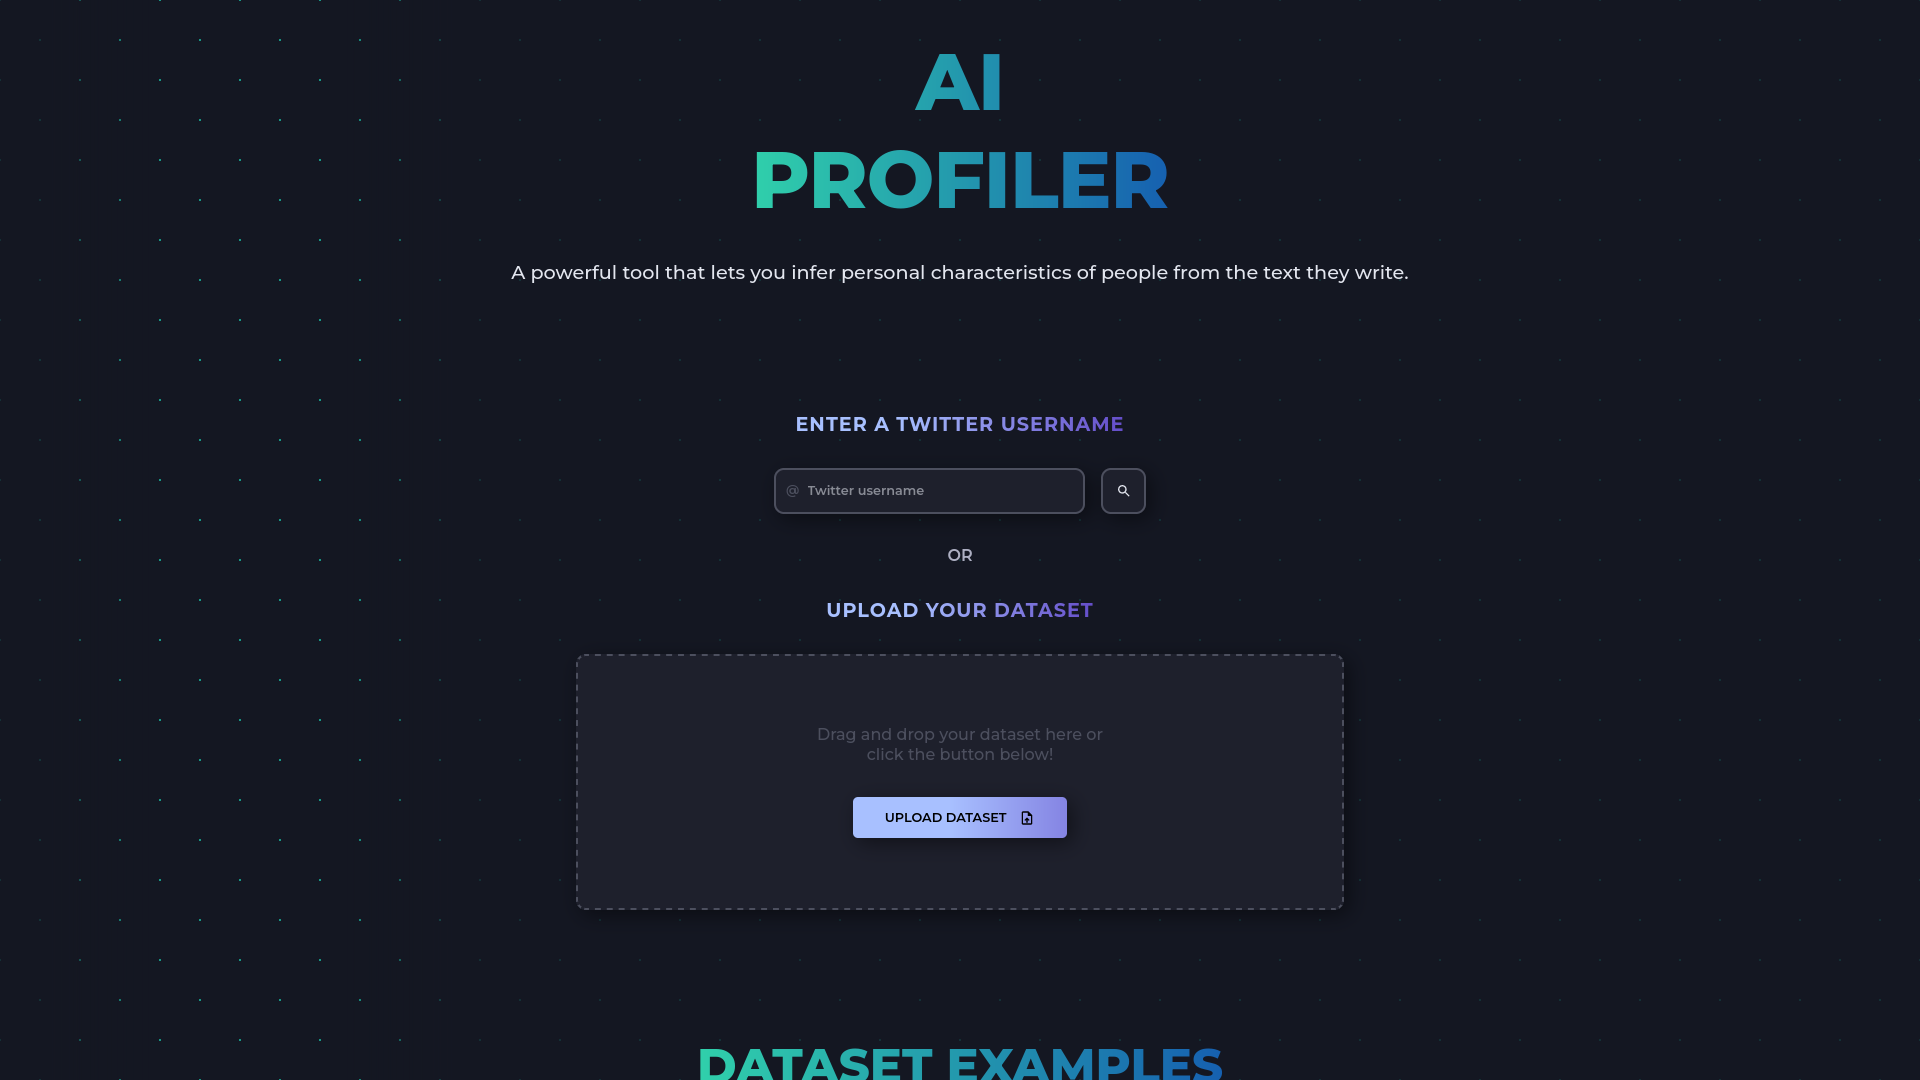
\includegraphics[width=\textwidth]{imagenes/home.png}
		\label{fig:casouso_home_escritorio}
	\end{subfigure}
	\hfill
	\begin{subfigure}[c]{0.21\textwidth}
		\centering
		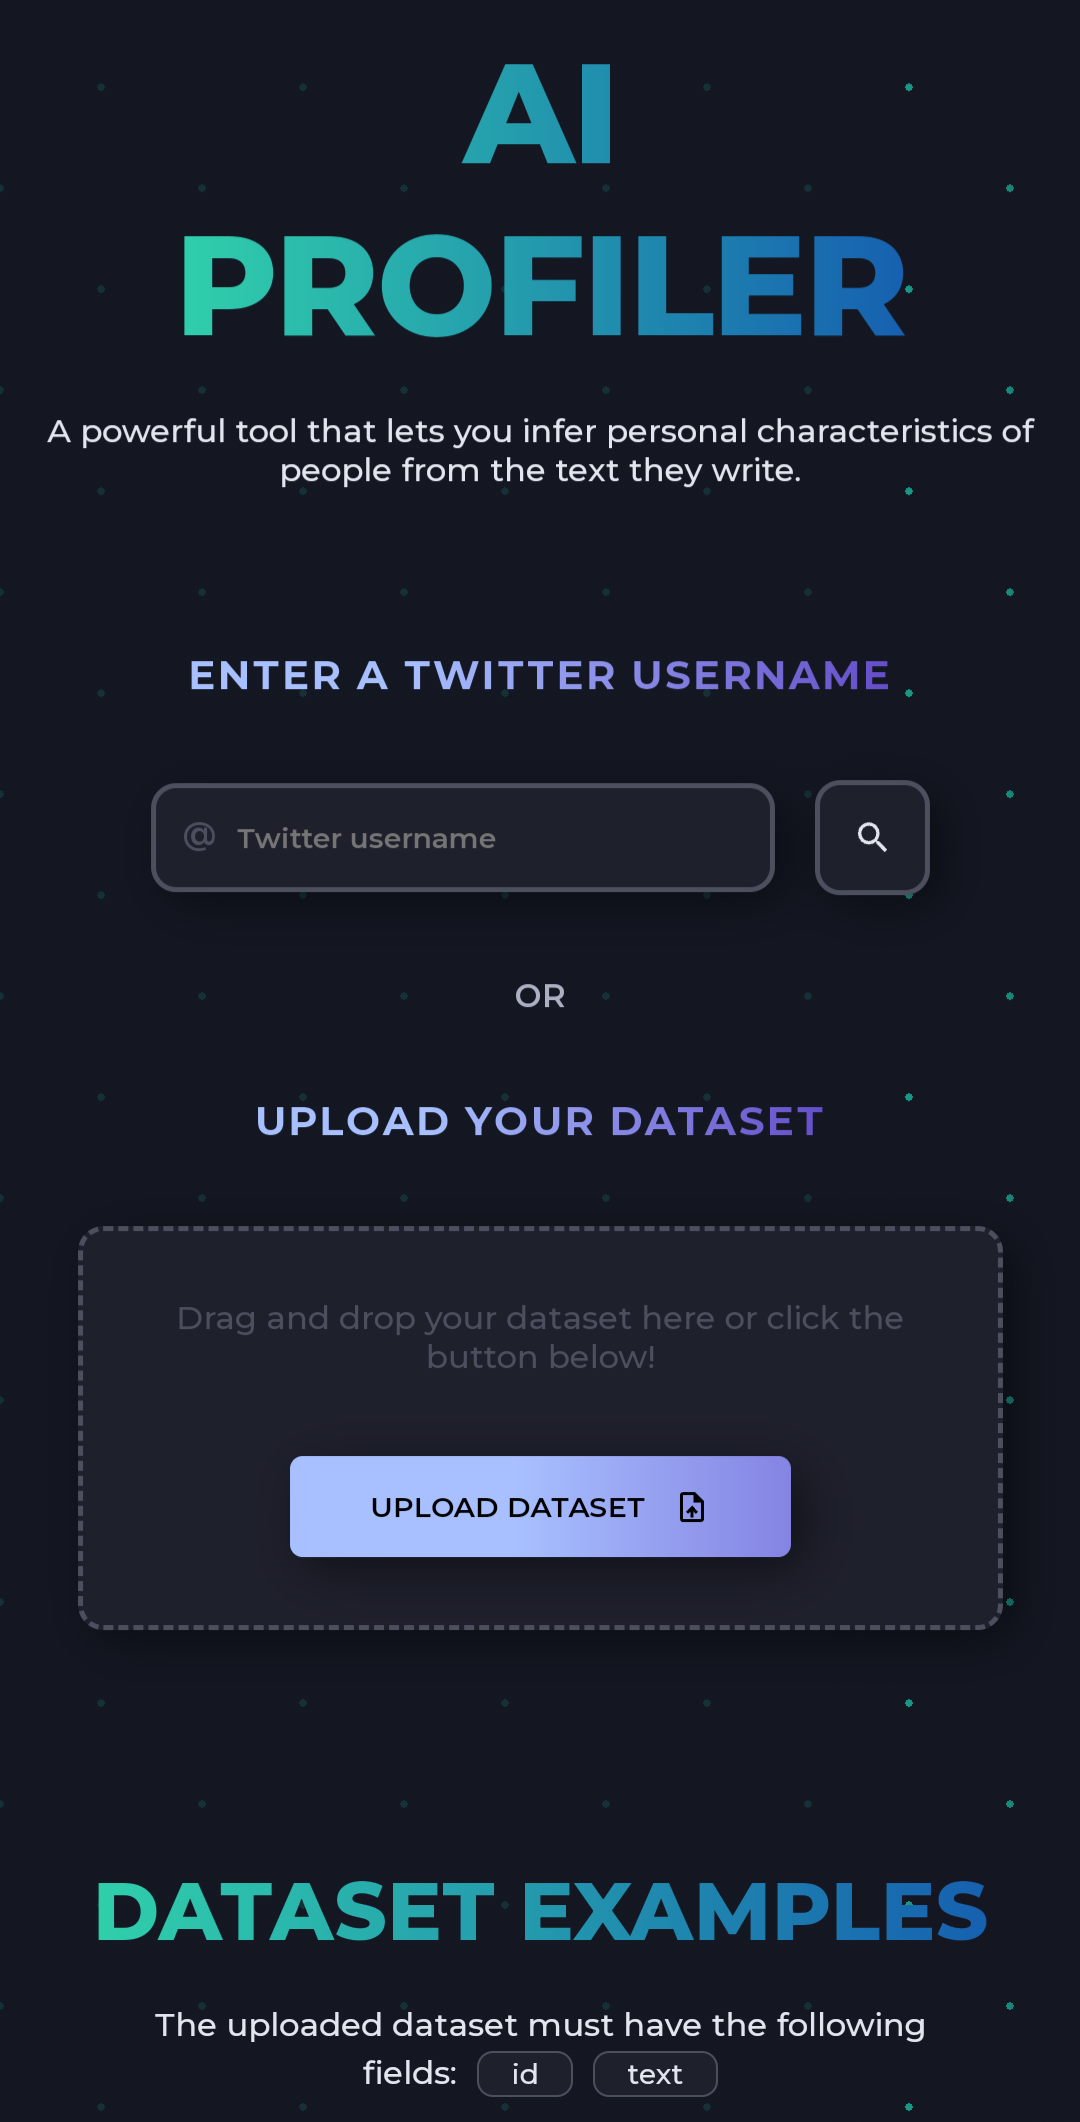
\includegraphics[width=\textwidth]{imagenes/home_movil.png}
		\label{fig:casouso_home_movil}
	\end{subfigure}
	\vspace{-1\baselineskip}
	\caption{Página de inicio de la aplicación}
	\label{fig:casouso_home}
\end{figure}

\bigskip
Asimismo, si el usuario desea conocer cual es la estructura y los campos que debe contener el \textit{dataset} que va a subir,
puede hacerlo consultando la sección de ejemplos, mostrada en la Figura \ref{fig:casouso_examples}, visible tras hacer \textit{scroll}
en la misma página de inicio.

\bigskip
\begin{figure}[H]
	\centering
	\begin{subfigure}[c]{0.74\textwidth}
		\centering
		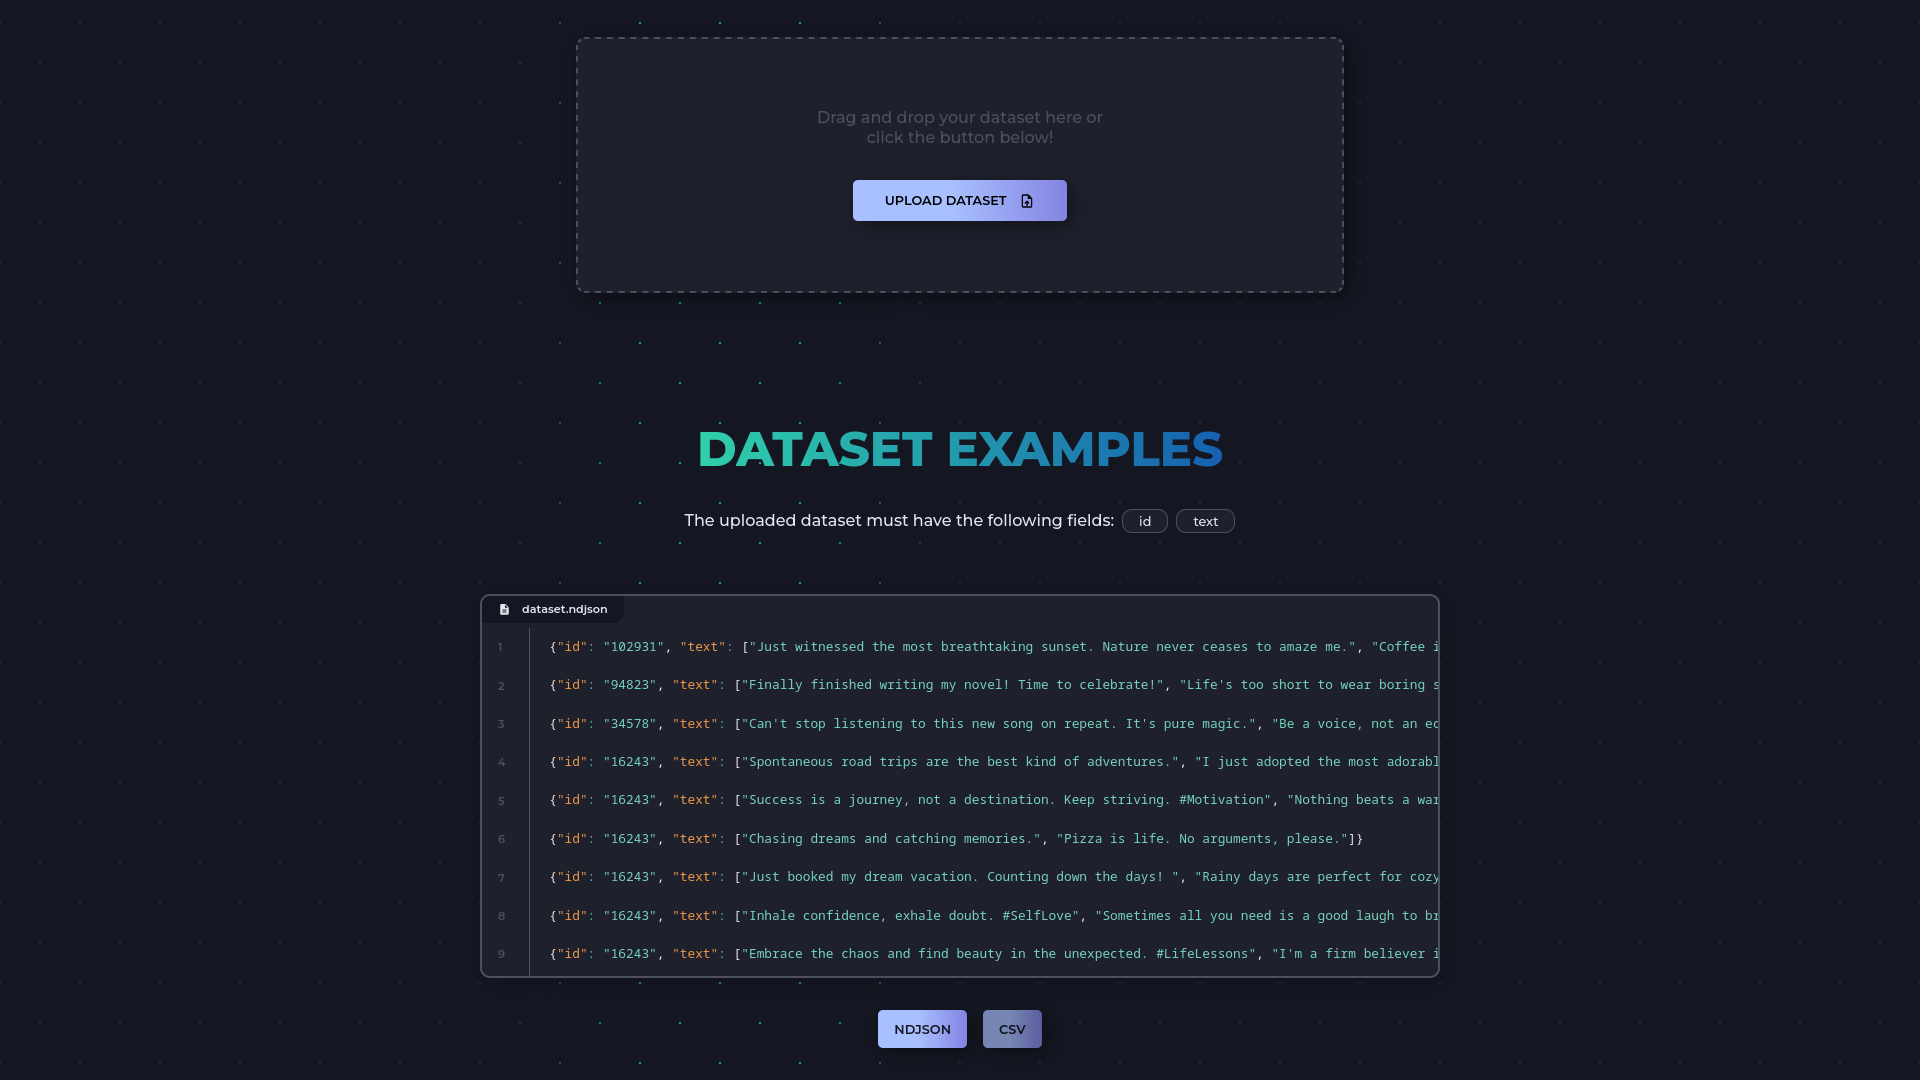
\includegraphics[width=\textwidth]{imagenes/examples.png}
		\label{fig:casouso_examples_escritorio}
	\end{subfigure}
	\hfill
	\begin{subfigure}[c]{0.21\textwidth}
		\centering
		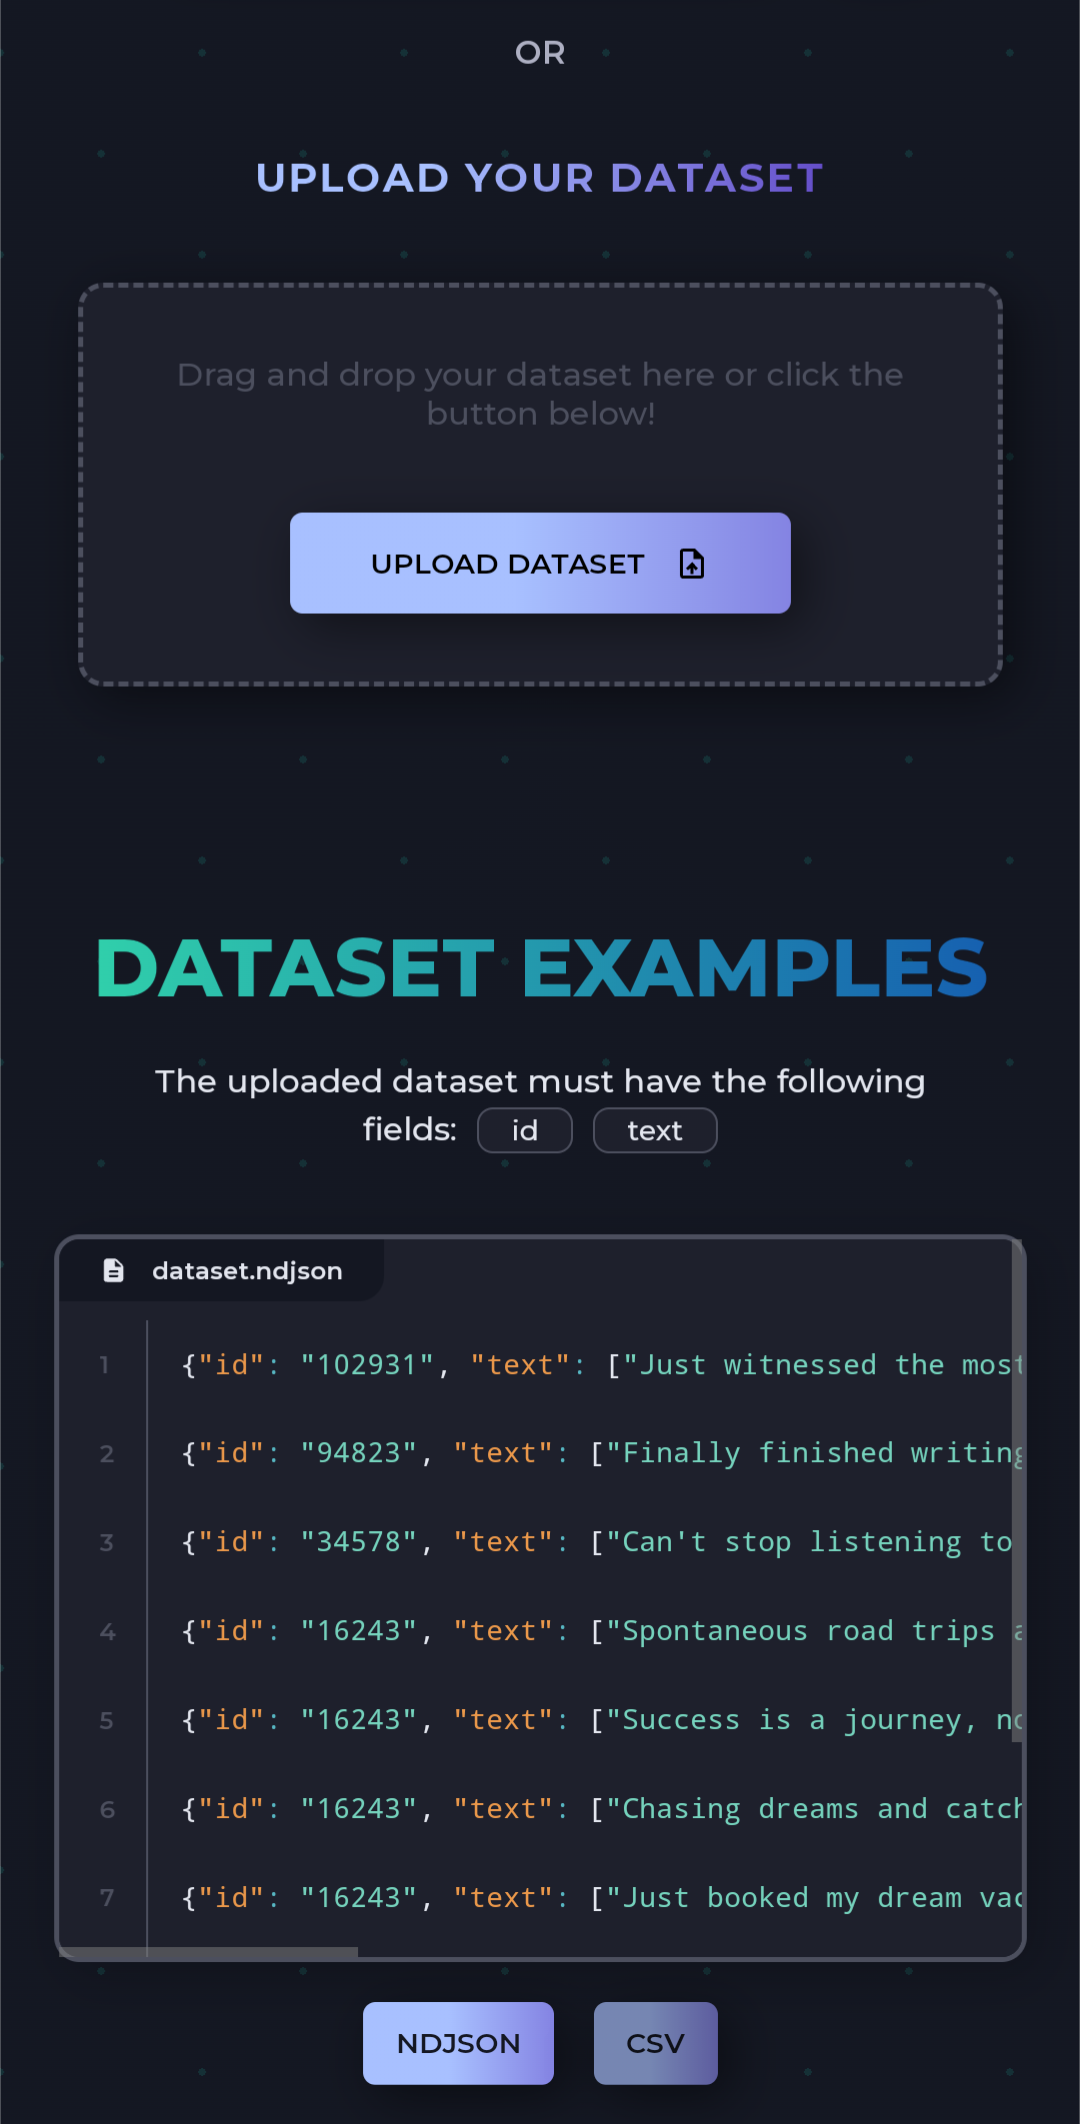
\includegraphics[width=\textwidth]{imagenes/examples_movil.png}
		\label{fig:casouso_examples_movil}
	\end{subfigure}
	\vspace{-1\baselineskip}
	\caption{Página de ejemplos de \textit{datasets}}
	\label{fig:casouso_examples}
\end{figure}

\section{Selección del algoritmo}
\label{sec:casouso_algoritmo}

En este punto, una vez subido el \textit{dataset} deseado, el usuario debe seleccionar el algoritmo de perfilado que más se ajuste
a sus necesidades. En este decisión, es fundamental tener en cuenta el lenguaje en el que se encuentra el \textit{dataset},
las características que se buscan perfilar, el rendimiento del algoritmo o incluso el \textit{dataset} con el que ha sido entrenado.
Así, por un lado se muestran unas tarjetas con la información básica de cada algoritmo, como se puede ver
en la Figura \ref{fig:casouso_algorithms} y, por otro lado, se muestran \textit{tooltips} con información más detallada
sobre el funcionamiento del algoritmo, el \textit{dataset} de entrenamiento y el rendimiento del mismo,
como se distingue en la Figura \ref{fig:casouso_tooltip}.

\bigskip
\begin{figure}[H]
	\centering
	\begin{subfigure}[c]{0.74\textwidth}
		\centering
		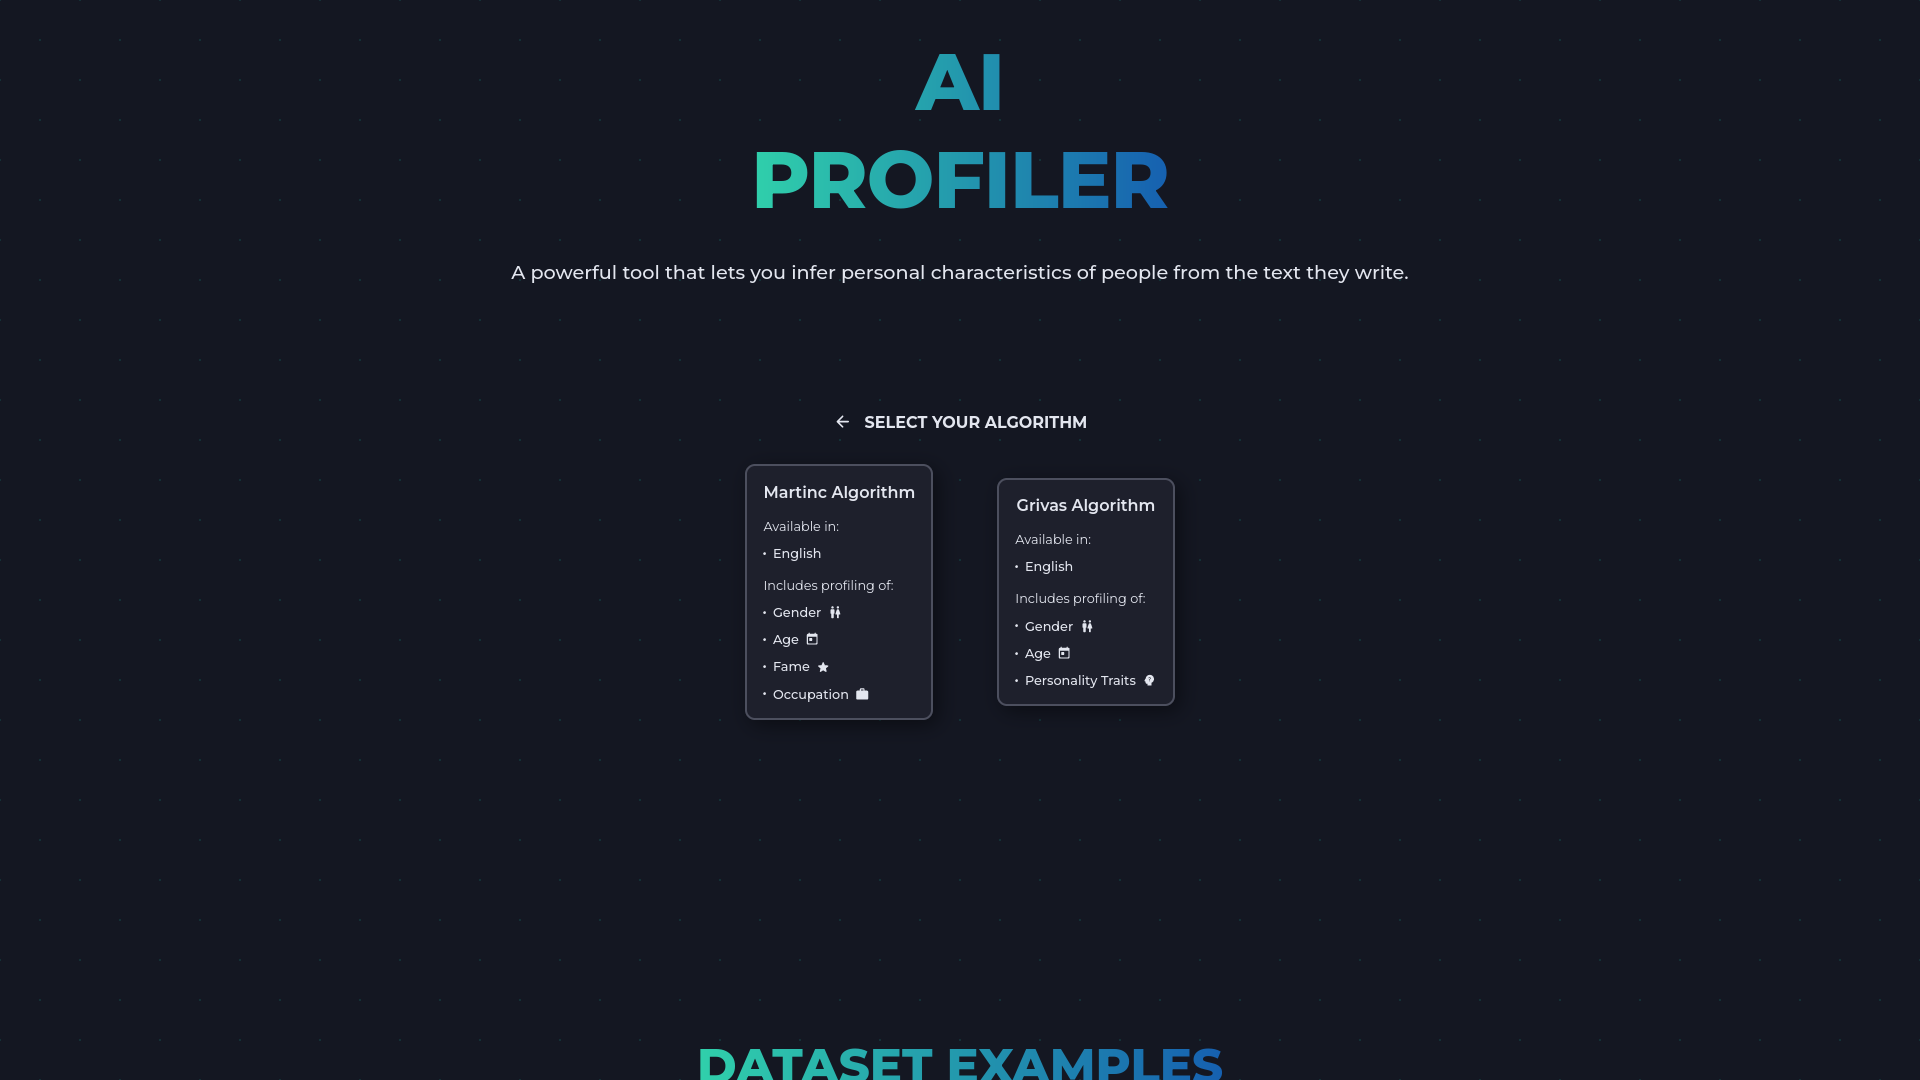
\includegraphics[width=\textwidth]{imagenes/algorithms.png}
		\label{fig:casouso_algorithms_escritorio}
	\end{subfigure}
	\hfill
	\begin{subfigure}[c]{0.21\textwidth}
		\centering
		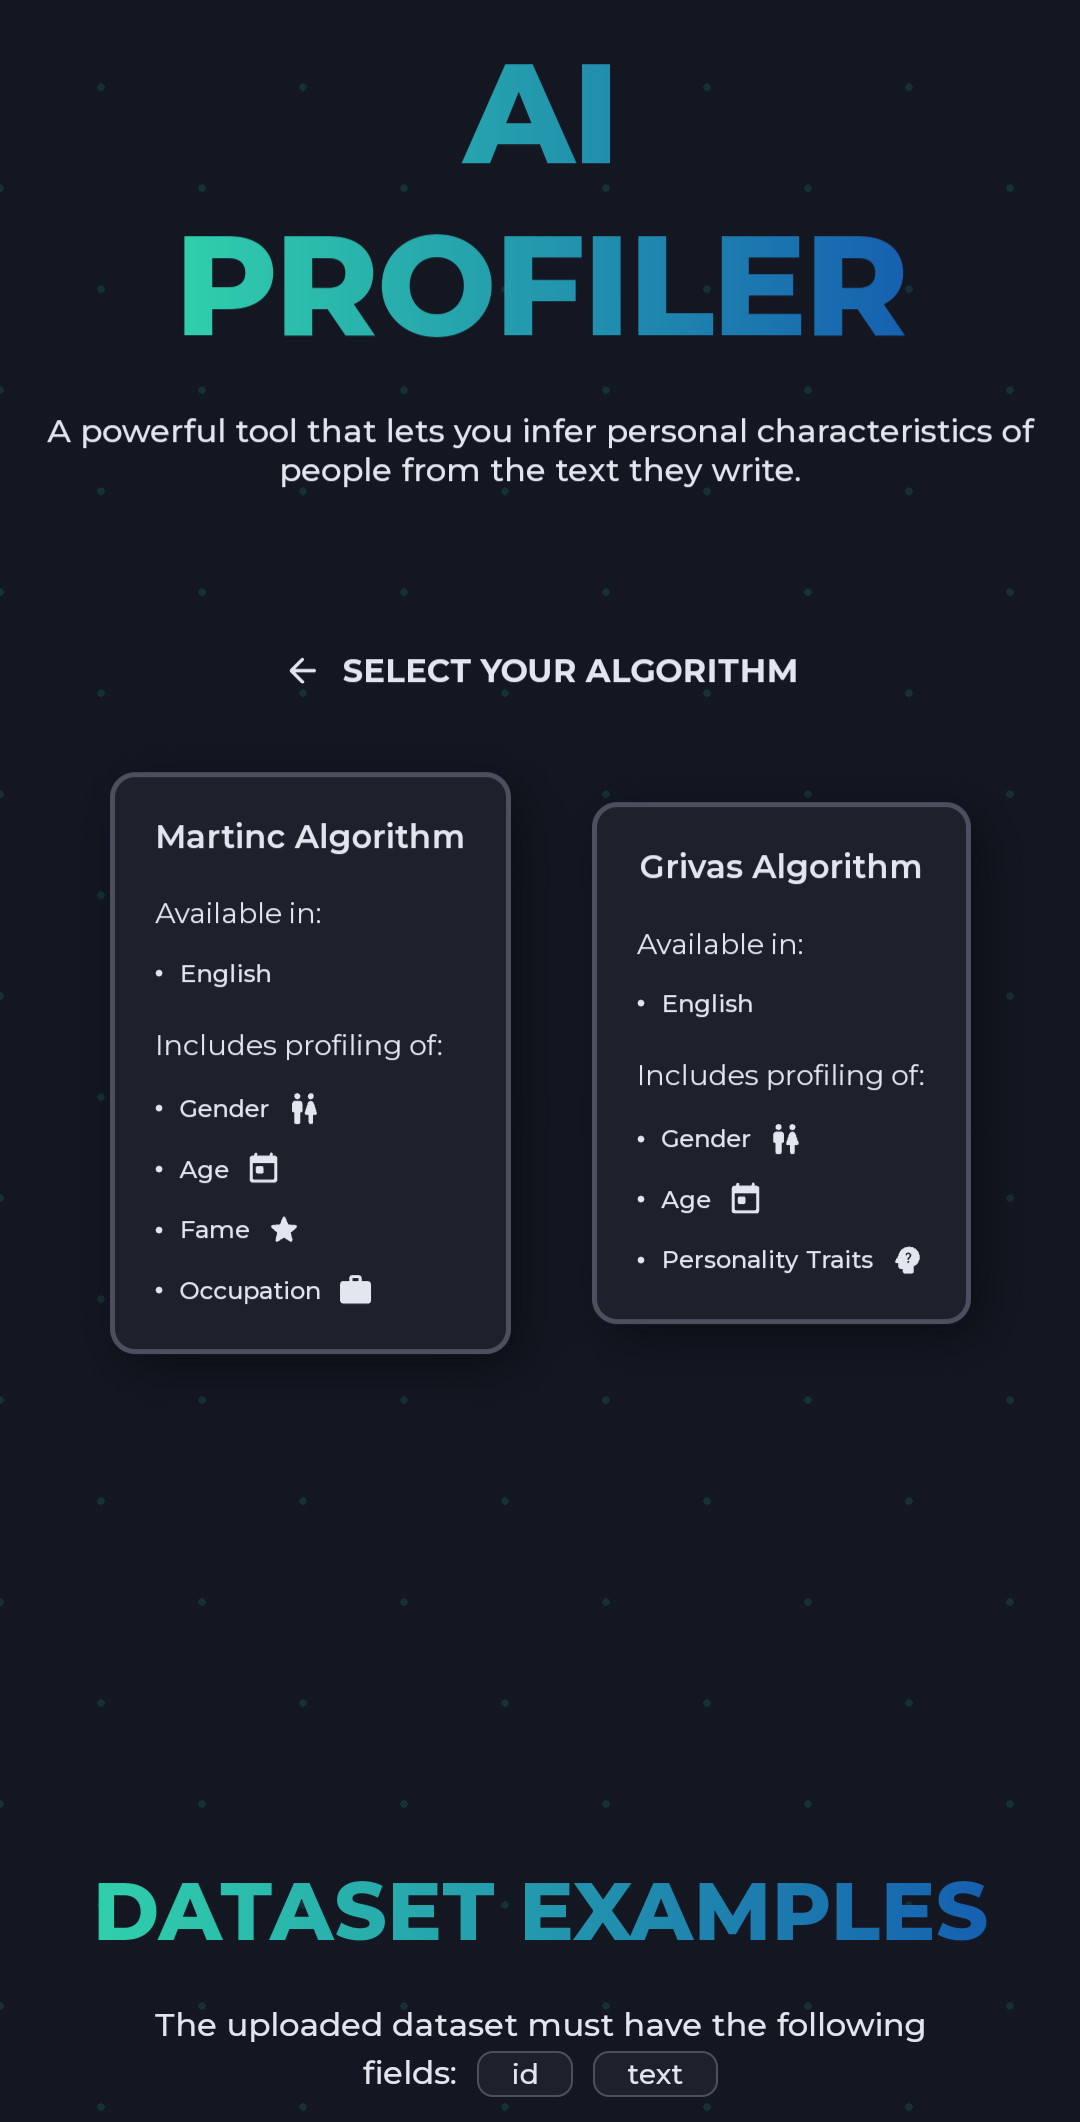
\includegraphics[width=\textwidth]{imagenes/algorithms_movil.png}
		\label{fig:casouso_algorithms_movil}
	\end{subfigure}
	\vspace{-1\baselineskip}
	\caption{Página de selección algoritmos}
	\label{fig:casouso_algorithms}
\end{figure}

\bigskip

\begin{figure}[H]
	\centering
	\begin{subfigure}[c]{0.50\textwidth}
		\centering
		\begin{tikzpicture}
			\node [inner sep=0pt] at (0,0) {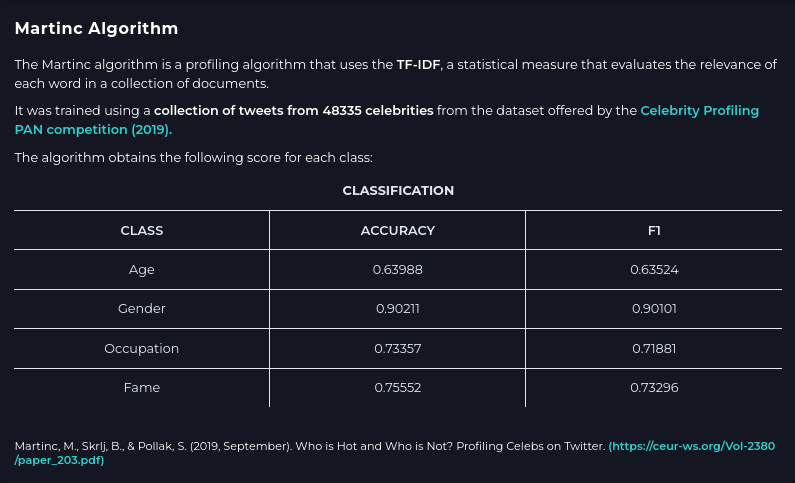
\includegraphics[width=\textwidth, keepaspectratio]{imagenes/tooltip-martinc.png}};
			\draw [appbg, line width=0.2cm]
			(current bounding box.north west) --
			(current bounding box.north east) --
			(current bounding box.south east) --
			(current bounding box.south west) -- cycle
			;
		\end{tikzpicture}
		\label{fig:casouso_tooltip_martinc}
	\end{subfigure}
	\hfill
	\begin{subfigure}[c]{0.455\textwidth}
		\centering
		\begin{tikzpicture}
			\node [inner sep=0pt] at (0,0) {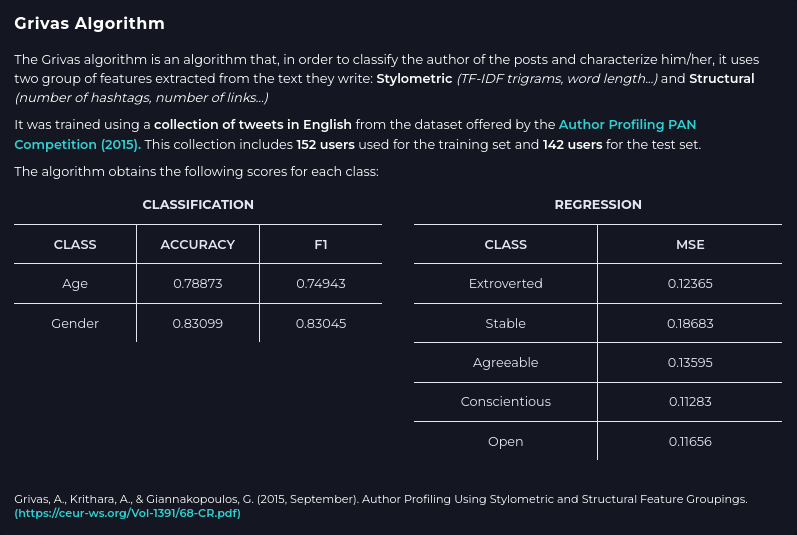
\includegraphics[width=\textwidth, keepaspectratio]{imagenes/tooltip-grivas.png}};
			\draw [appbg, line width=0.2cm]
			(current bounding box.north west) --
			(current bounding box.north east) --
			(current bounding box.south east) --
			(current bounding box.south west) -- cycle
			;
		\end{tikzpicture}
		\label{fig:casouso_tooltip_grivas}
	\end{subfigure}
	\vspace{-1\baselineskip}
	\caption{Tooltip de información sobre los algoritmos}
	\label{fig:casouso_tooltip}
\end{figure}

\section{Proceso de perfilado}
\label{sec:casouso_perfilado}

Después de seleccionar el algoritmo, se muestra una página a modo de resumen, en la que se puede observar el \textit{dataset} subido
junto al algoritmo seleccionado. Para comenzar el proceso de perfilado, el usuario debe pulsar el botón
\textit{Start profiling} y, para proporcionar \textit{feedback} sobre la ejecución del proceso y mejorar la experiencia de usuario,
se muestra una barra de progreso infinita. Esta página puede verse en la Figura \ref{fig:casouso_overview}.

\bigskip
\begin{figure}[H]
	\centering
	\begin{subfigure}[c]{0.74\textwidth}
		\centering
		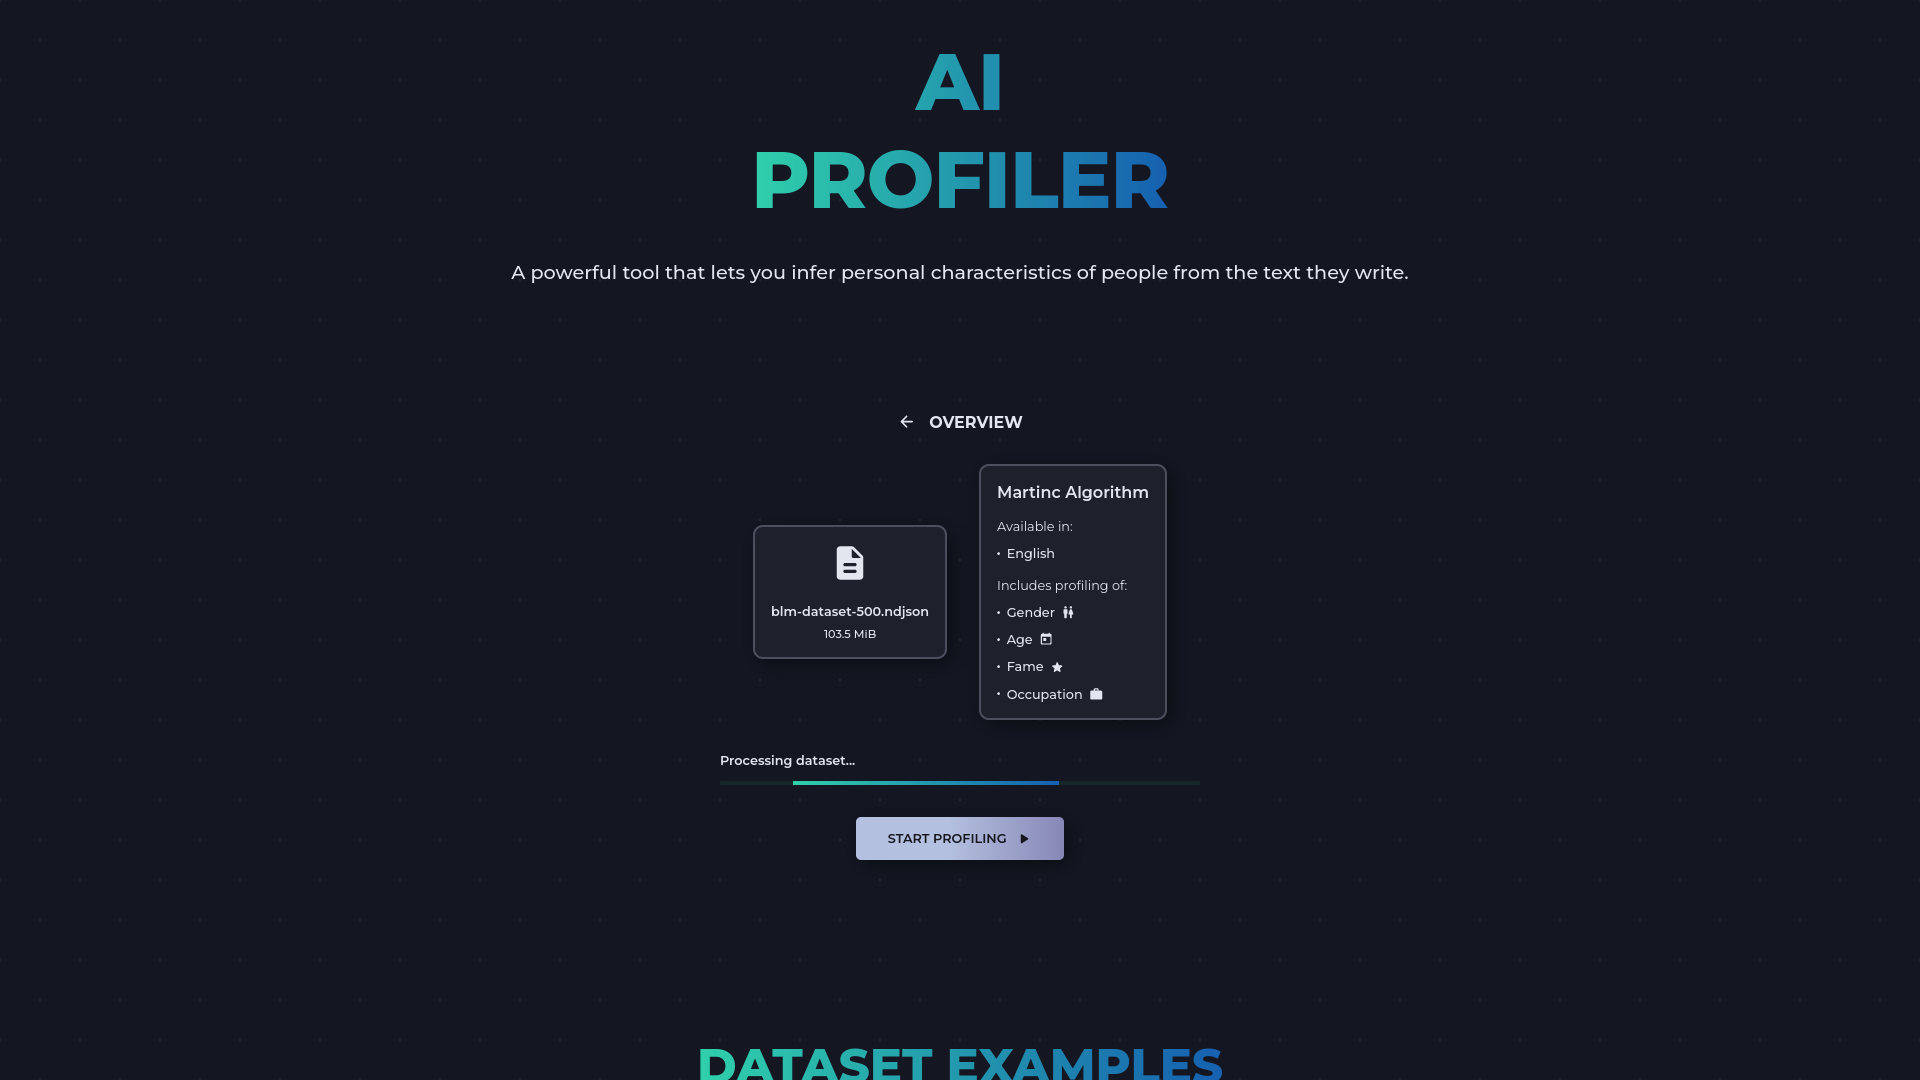
\includegraphics[width=\textwidth]{imagenes/overview.png}
		\label{fig:casouso_overview_escritorio}
	\end{subfigure}
	\hfill
	\begin{subfigure}[c]{0.21\textwidth}
		\centering
		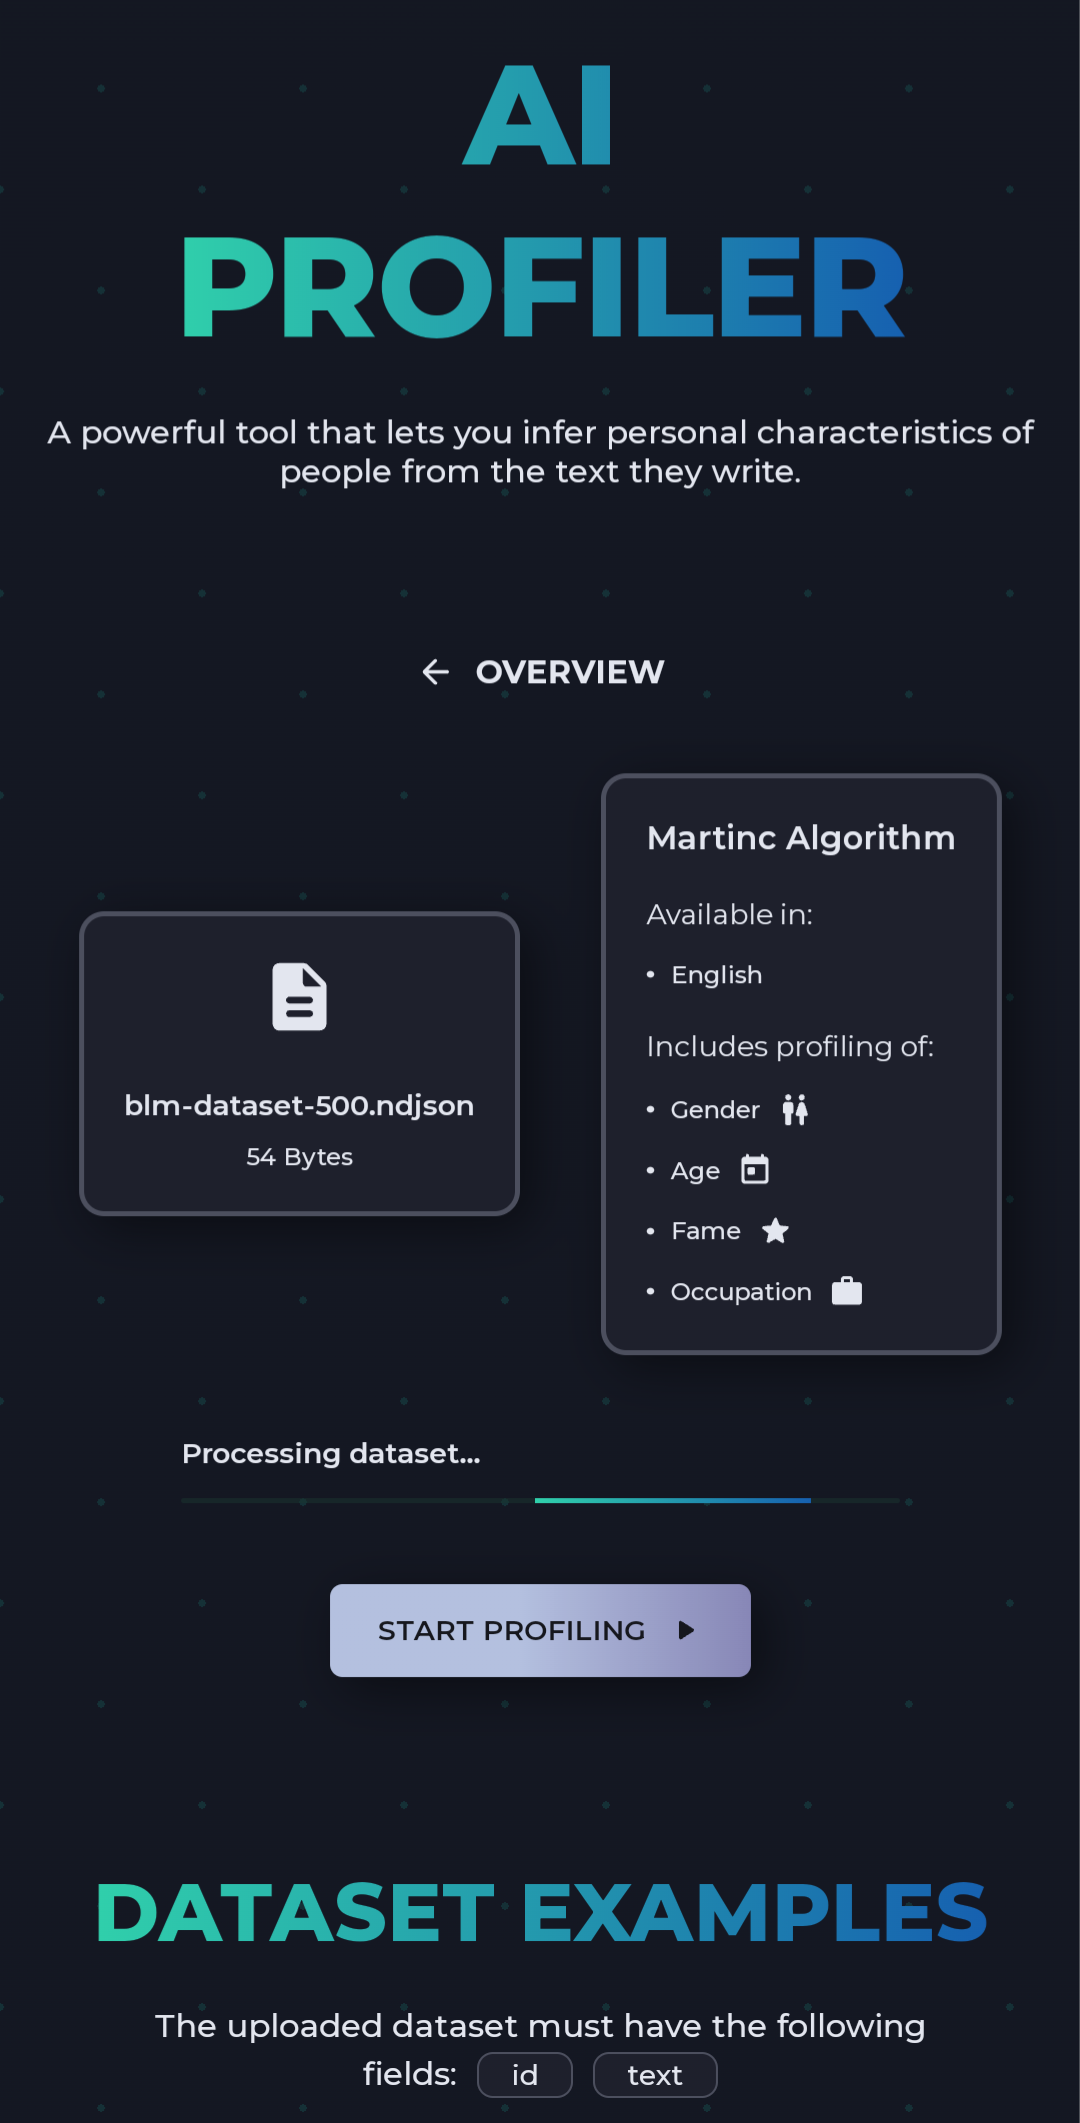
\includegraphics[width=\textwidth]{imagenes/overview_movil.png}
		\label{fig:casouso_overview_movil}
	\end{subfigure}
	\vspace{-1\baselineskip}
	\caption{Página de resumen del perfilado}
	\label{fig:casouso_overview}
\end{figure}

\section{Visualización de resultados}
\label{sec:casouso_dashboard}

Tras finalizar el proceso de perfilado, se muestra una página con los resultados obtenidos en formato \textit{dashboard}, al igual
que se especificaba en los prototipos de la Sección \ref{sec:diseño_prototipado}. De esta forma, el \textit{dashboard} fue
implementado teniendo como objetivo principal que toda la información estuviera disponible en una única página en la que se
mostraran únicamente datos relevantes para el usuario, sin necesidad de hacer \textit{scroll} para verla. Asimismo, en función del algoritmo
empleado, se muestran unos gráficos u otros, como se puede ver en las Figuras \ref{fig:casouso_dashboard_martinc} y
\ref{fig:casouso_dashboard_grivas}.

\bigskip
\begin{figure}[H]
	\centering
	\begin{subfigure}[c]{0.74\textwidth}
		\centering
		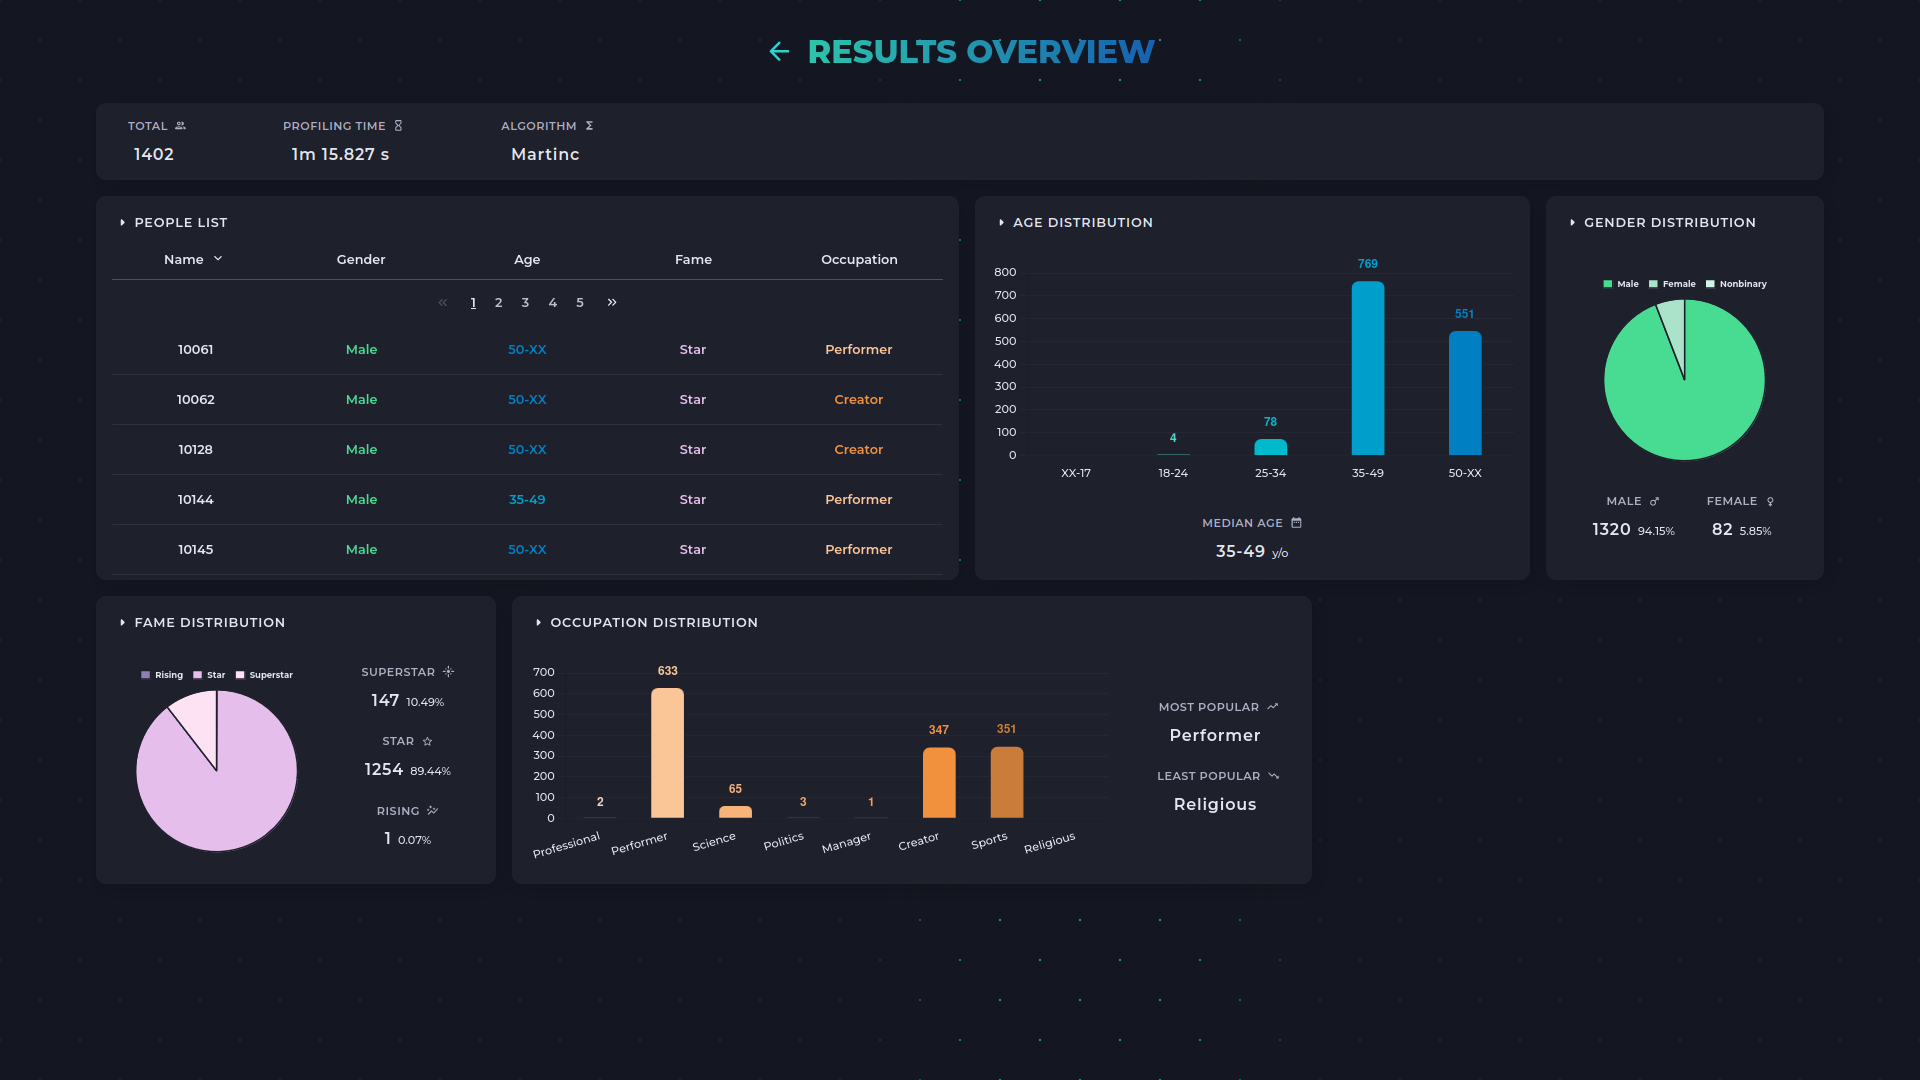
\includegraphics[width=\textwidth]{imagenes/dashboard-martinc-500.png}
		\label{fig:casouso_dashboard_martinc_escritorio}
	\end{subfigure}
	\hfill
	\begin{subfigure}[c]{0.21\textwidth}
		\centering
		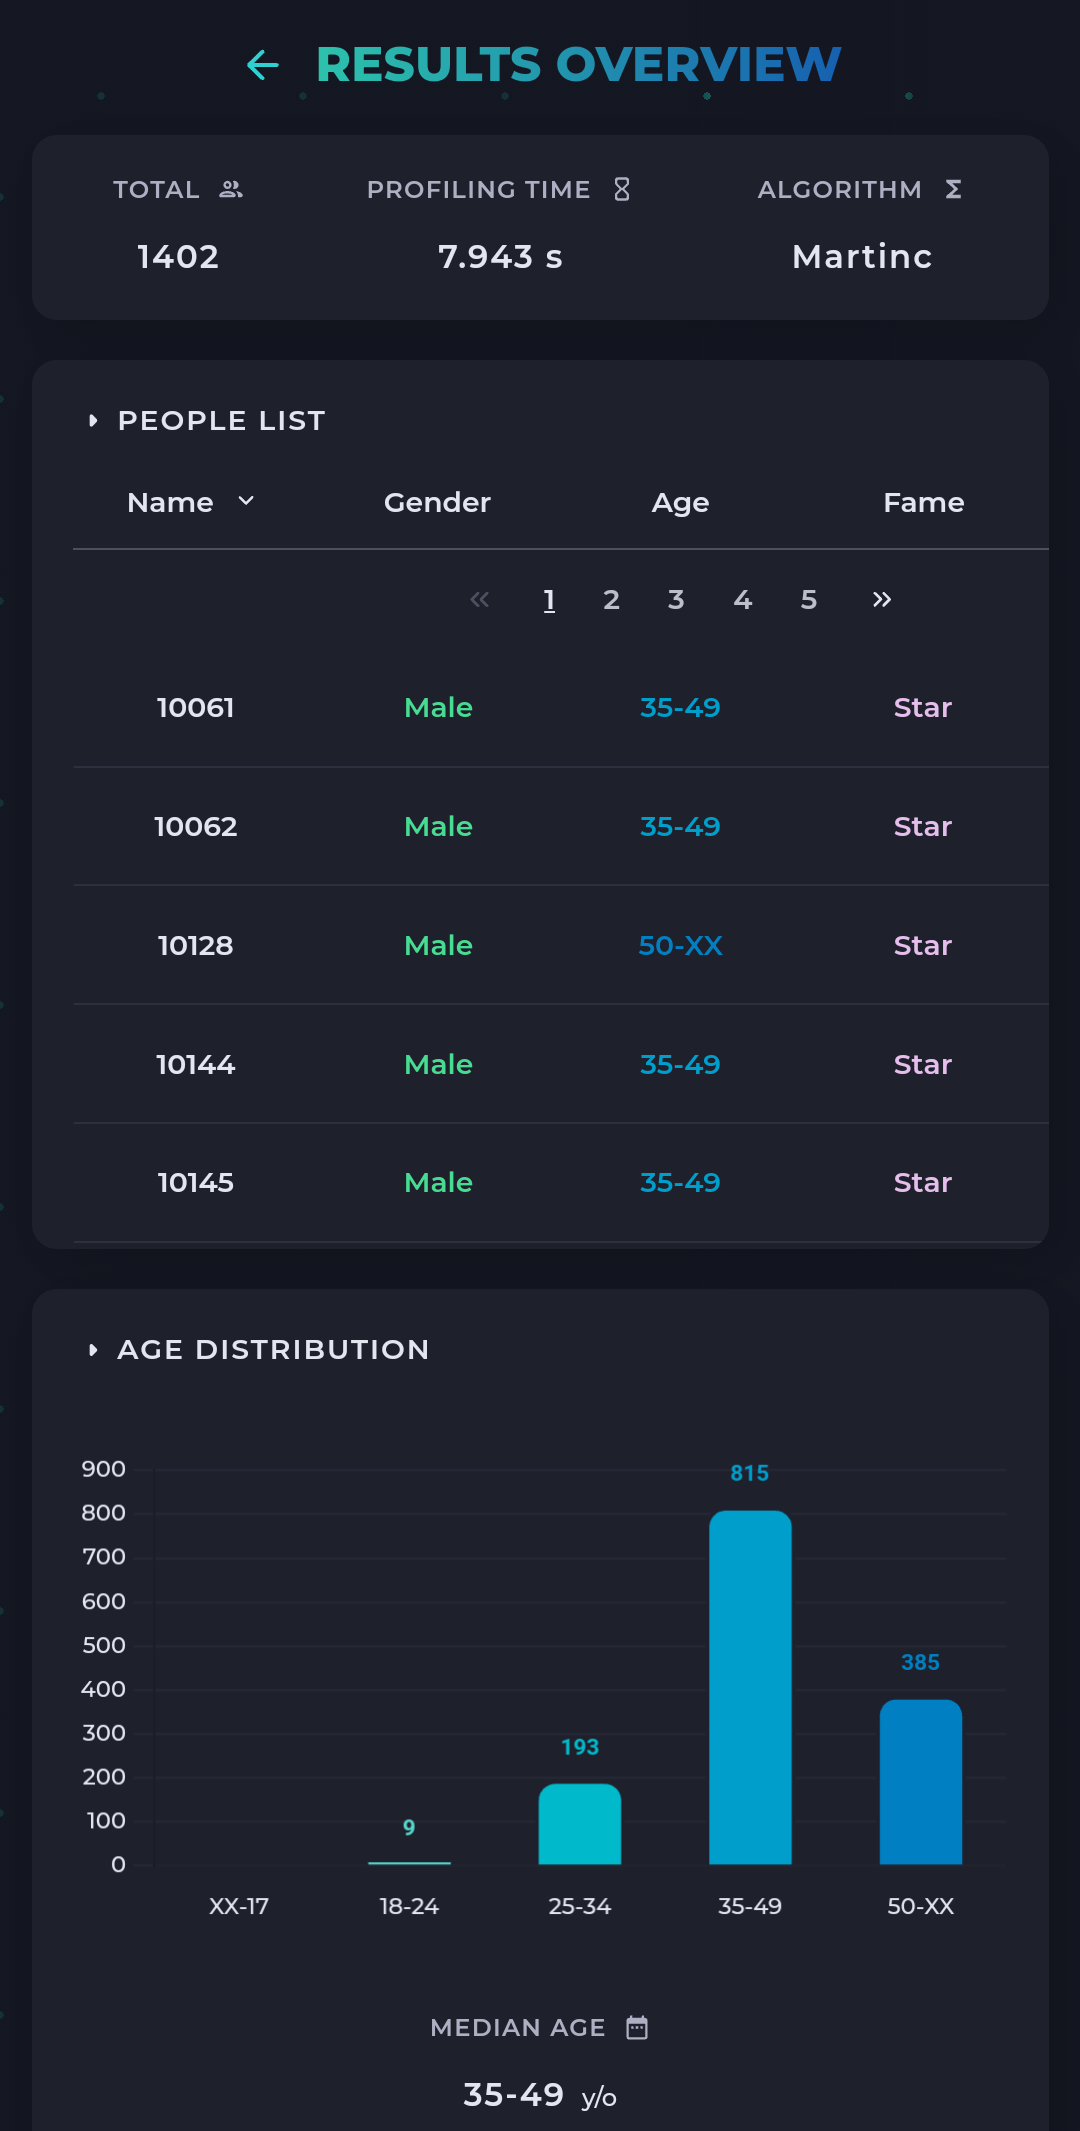
\includegraphics[width=\textwidth]{imagenes/dashboard-martinc-500_movil.png}
		\label{fig:casouso_dashboard_martinc_movil}
	\end{subfigure}
	\vspace{-1\baselineskip}
	\caption{\textit{Dashboard} con los resultados obtenidos por el algoritmo de Martinc \cite{martinc2019hot}}
	\label{fig:casouso_dashboard_martinc}
\end{figure}

\begin{figure}[H]
	\centering
	\begin{subfigure}[c]{0.74\textwidth}
		\centering
		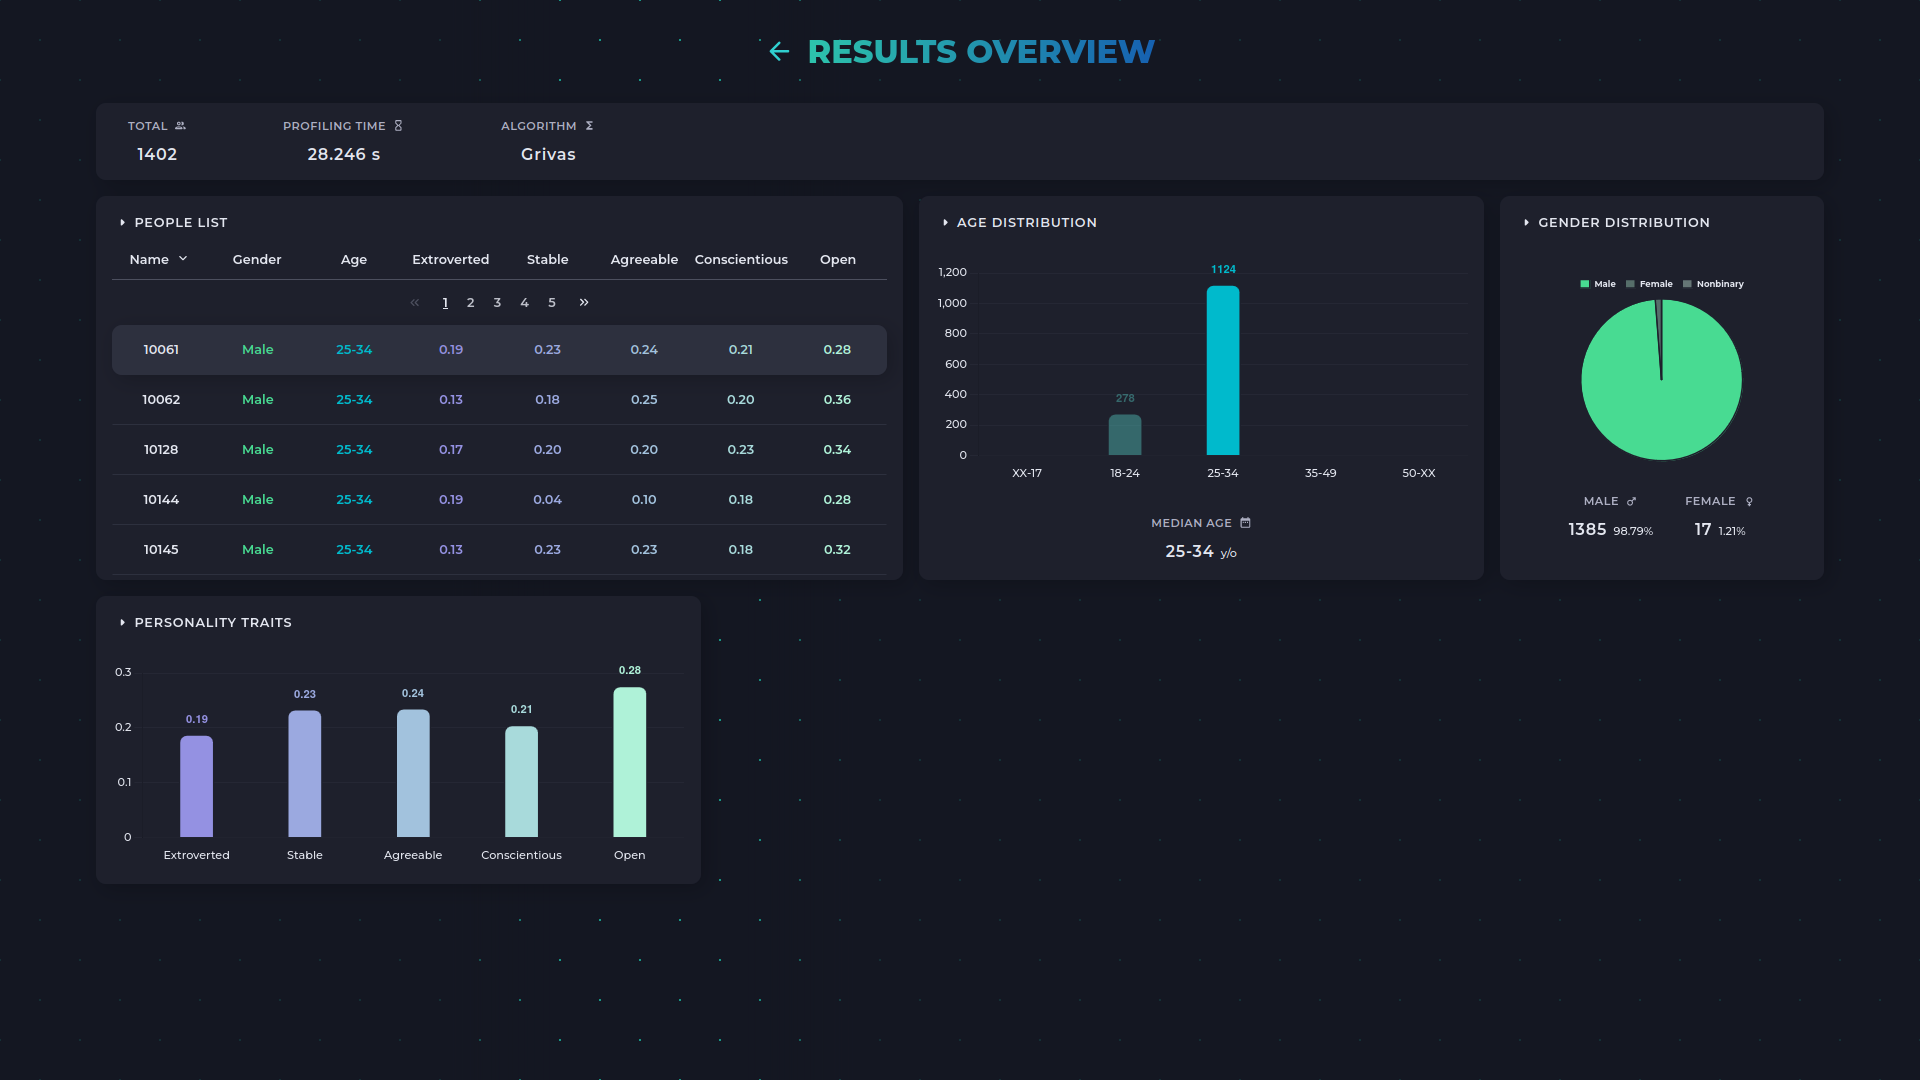
\includegraphics[width=\textwidth]{imagenes/dashboard-grivas-500.png}
		\label{fig:casouso_dashboard_grivas_escritorio}
	\end{subfigure}
	\hfill
	\begin{subfigure}[c]{0.21\textwidth}
		\centering
		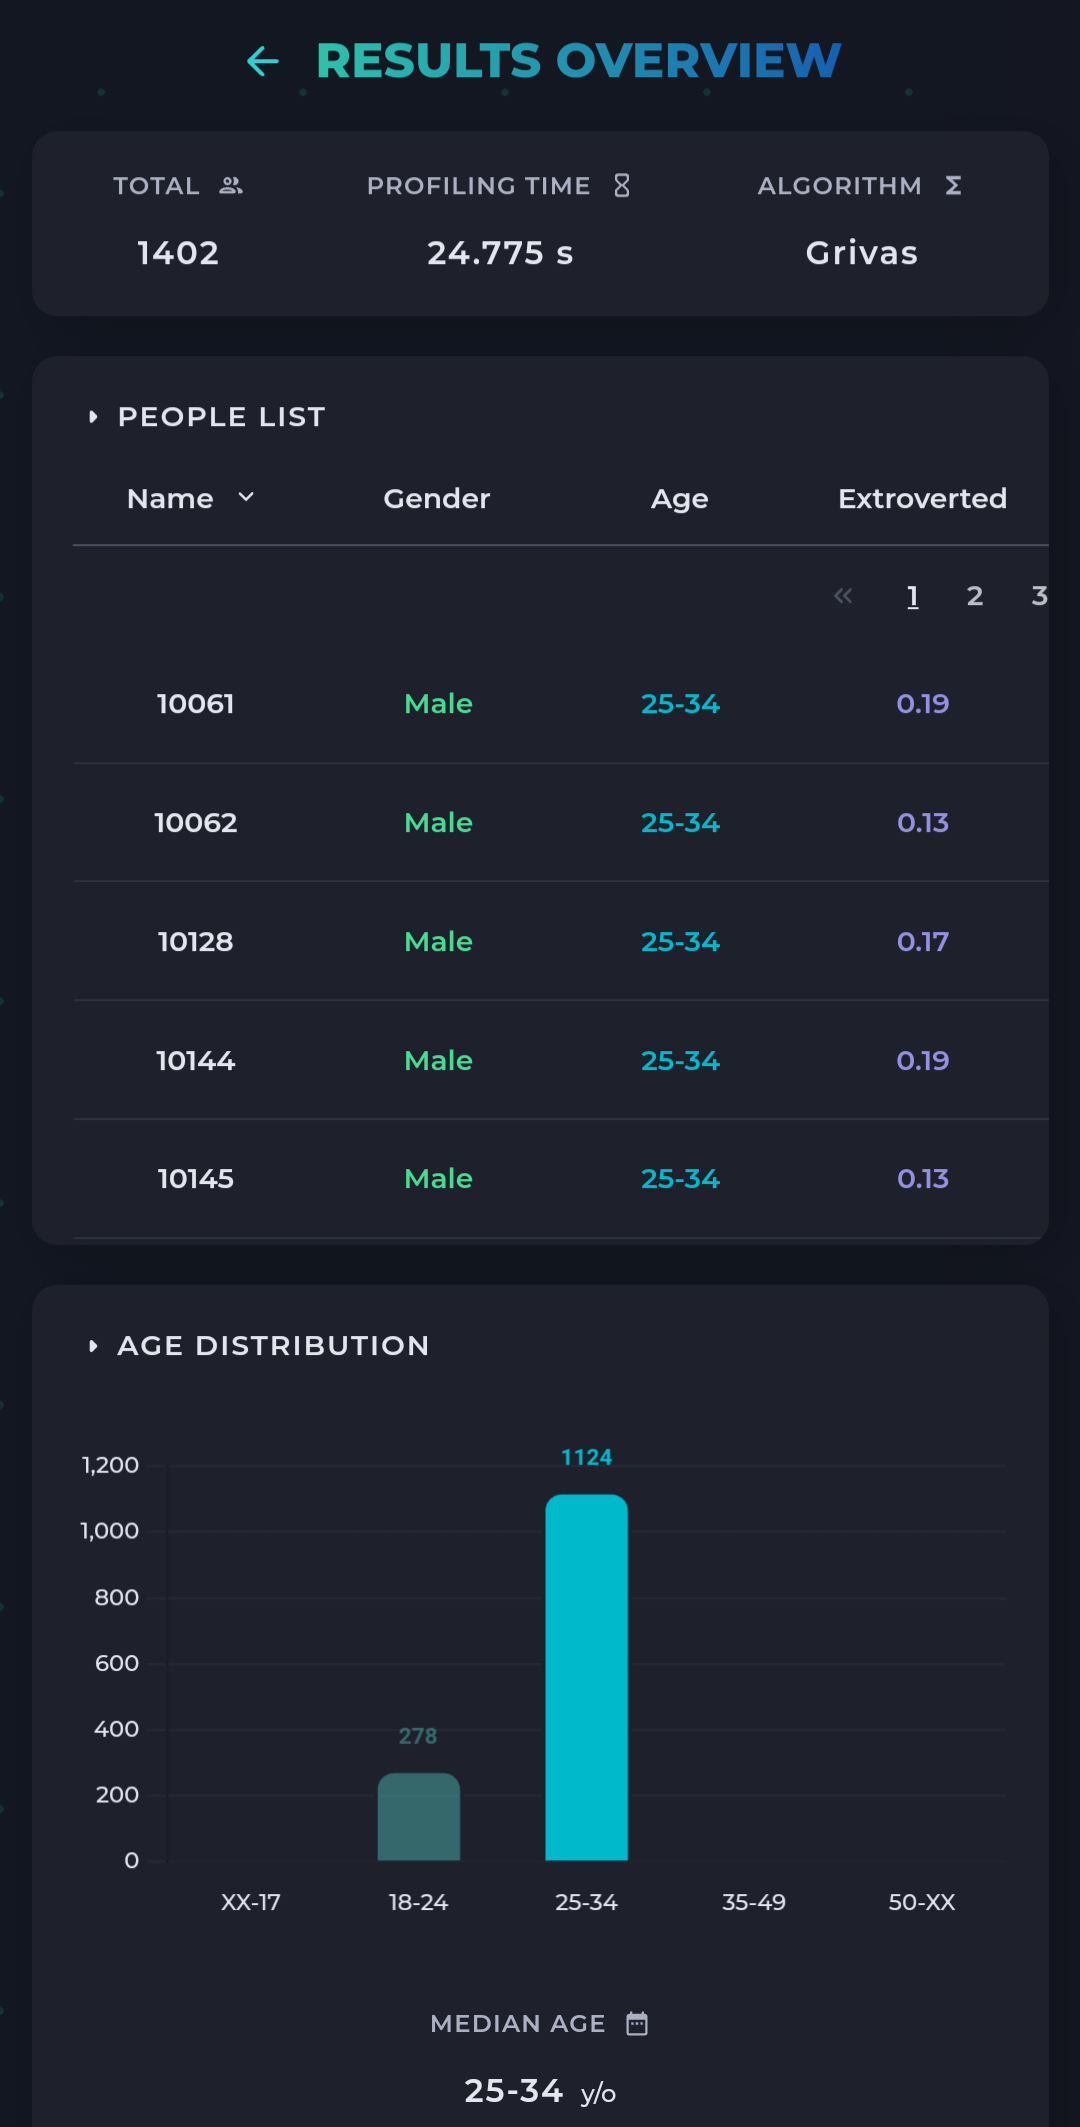
\includegraphics[width=\textwidth]{imagenes/dashboard-grivas-500_movil.png}
		\label{fig:casouso_dashboard_grivas_movil}
	\end{subfigure}
	\vspace{-1\baselineskip}
	\caption{\textit{Dashboard} con los resultados obtenidos por el algoritmo de Grivas \cite{grivas2015author}}
	\label{fig:casouso_dashboard_grivas}
\end{figure}

\section{Análisis de resultados}
\label{sec:casouso_analisis}

Para llevar a cabo el análisis de los resultados obtenidos, se abordará el estudio de cada característica por separado desde un marco sociológico y se
compararán las predicciones realizadas por ambos algoritmos. A mayores, y a modo de experimentación para comprobar las diferencias subyacentes en el perfilado,
se hará uso de tres \textit{datasets} con diferente número de posts por usuario, como se comentó en la Sección \ref{sec:casouso_dataset}.

\subsection{Distribución de género}
\label{subsec:casouso_analisis_genero}

En cuanto a la distribución de género, como se aprecia en la Tabla \ref{tab:comparativa_genero}, ambos algoritmos otorgan una gran mayoría al género masculino en cualquiera de
los tres \textit{datasets}.

\bigskip
En el caso del algoritmo de Grivas \cite{grivas2015author}, observamos como, a medida que aumenta el número de posts por usuario,
el número de usuarios clasificados como femeninos disminuye drásticamente. Como ya se adelantó en la Sección \ref{sec:pan_2015_corpus}, este fenómento se debe a que el \textit{dataset} utilizado para entrenar
dicho algoritmo era muy limitado, de apenas 150 personas, por lo que no es lo suficientemente representativo y no generaliza de forma óptima.

\bigskip
En lo que respecta al algoritmo de Martinc \cite{martinc2019hot}, vemos como, al aumentar el número de posts por usuario, aquellos clasificados como masculinos
se estabilizan alrededor de 1,320 (94\%), mientras que aquellos clasificados como femeninos se quedan en 82 (6\%).
Estos resultados, a simple vista, no tienen una relación clara con la realidad dado que, según Statista, la distribución de género en Reddit es
de un 64\% para los hombres y un 36\% para las mujeres \cite{statistagenero}.
Sin embargo, es importante resaltar que la proporción de género puede variar ampliamente
en función del tema del que se esté hablando. Así, como recoge Thelwall et al., 2019 \cite{thelwall2019she}, existen amplias diferencias en cuanto a la participación
de cada género en temas políticos, y es que, la proporción de mujeres en \textit{subreddits} como \textit{Politics}, en el que se tratan temas de actualidad
política en Estados Unidos, es de tan solo un 20,5\%. A raíz de este hecho, podemos inferir que existió una menor participación de las mujeres en el movimiento \#BLM
en el marco de las redes sociales, lo que, a su vez, permite trazar como hipótesis de trabajo si en las manifestaciones y protestas
sucedidas en la vida real existía también una menor participación del género femenino.

\bigskip
Por otro lado, antendiendo a las limitaciones del propio modelo, podemos destacar el hecho de que el conjunto de entrenamiento está formado por \textit{tweets} de celebridades,
haciendo que pueda no ser directamente aplicable a cualquier conjunto de usuarios o redes sociales diferentes.

\bigskip
\begin{figure}[H]
	\centering
	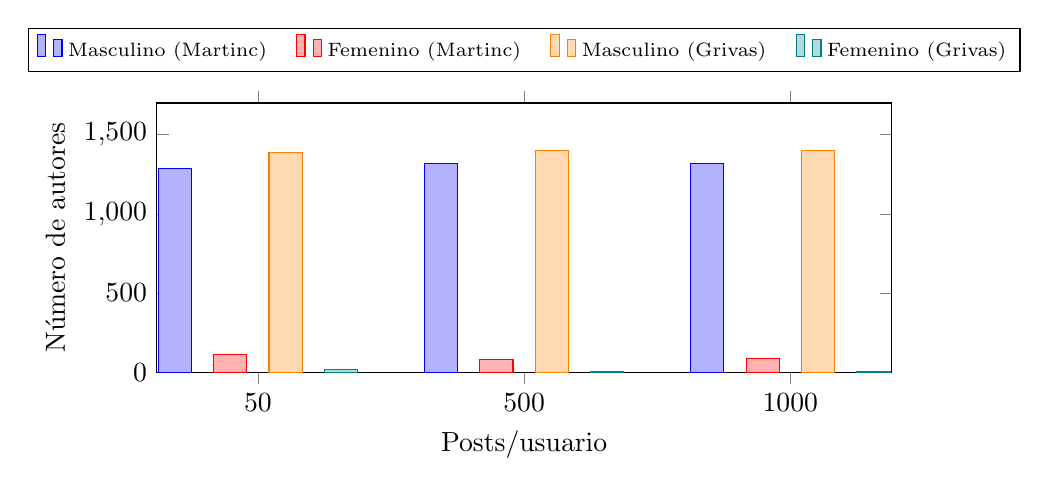
\begin{tikzpicture}
		\begin{axis}[
				width=0.9\textwidth,
				height=5cm,
				xmajorgrids=false,
				ylabel=Número de autores,
				xlabel=Posts/usuario,
				ybar=8pt,
				bar width=12pt,
				enlarge x limits=0.19,
				symbolic x coords={50, 500, 1000},
				xtick=data,
				ymin=0,
				ymax=1700,
				legend style={at={(0.5,1.28)},font=\scriptsize, anchor=north,legend columns=-1, /tikz/every even column/.append style={column sep=0.3cm}},
			]
			\addplot table[x=Posts/usuario,y={Masculino (Martinc)}] {
			Posts/usuario   {Masculino (Martinc)}
			50              1288
			500             1320
			1000            1318
			};
			\addplot table[x=Posts/usuario,y={Femenino (Martinc)}] {
			Posts/usuario   {Femenino (Martinc)}
			50              114
			500             82
			1000            84
			};
			\addplot[color=orange, fill=orange!30] table[x=Posts/usuario,y={Masculino (Grivas)}] {
			Posts/usuario   {Masculino (Grivas)}
			50              1385
			500             1400
			1000            1400
			};
			\addplot[color=teal, fill=teal!30] table[x=Posts/usuario,y={Femenino (Grivas)}] {
			Posts/usuario   {Femenino (Grivas)}
			50              17
			500             2
			1000            2
			};
			\legend{{Masculino (Martinc)}, {Femenino (Martinc)}, {Masculino (Grivas)}, {Femenino (Grivas)}}
		\end{axis}
	\end{tikzpicture}
	\caption{Distribución de género obtenida por ambos algoritmos}
	\label{fig:comparativa_genero}
\end{figure}


\bigskip
\begin{table}[H]
	\centering
	\resizebox{0.8\textwidth}{!}{
		\rowcolors{2}{white}{udcgray!25}
		\setlength{\tabcolsep}{0.6cm}
		\begin{tabular}{|c|c|c|c|c|}
			\hhline{~|----|}
			\multicolumn{1}{c|}{\cellcolor{white}}       & \multicolumn{2}{c|}{\cellcolor{udcpink!25}\textbf{Martinc}} & \multicolumn{2}{c|}{\cellcolor{udcpink!25}\textbf{Grivas}}              \\ \hline
			\multicolumn{1}{|c|}{\textbf{Posts/usuario}} & \multicolumn{1}{c|}{\textbf{Masculino}}                     & \multicolumn{1}{c|}{\textbf{Femenino}}                     &
			\multicolumn{1}{c|}{\textbf{Masculino}}      & \multicolumn{1}{c|}{\textbf{Femenino}}                                                                                                \\ \hline
			50                                           & 1.288                                                       & 114                                                        & 1.385 & 17 \\ \hline
			500                                          & 1.315                                                       & 87                                                         & 1.400 & 2  \\ \hline
			1.000                                        & 1.318                                                       & 84                                                         & 1.400 & 2  \\ \hline
		\end{tabular}
	}
	\caption{Distribución de género obtenida por ambos algoritmos}
	\label{tab:comparativa_genero}
\end{table}

\subsection{Distribución de edad}
\label{subsec:casouso_analisis_edad}

En el caso de la distribución de edad, ambos algoritmos reflejan amplias diferencias en los resultados obtenidos, como se puede
ver en las Tablas \ref{tab:comparativa_edad_martinc} y \ref{tab:comparativa_edad_grivas}.

\bigskip
Para el algoritmo de Martinc et al. \cite{martinc2019hot}, observamos
como, a medida que aumenta el número de posts por usuario, el número de usuarios pertenecientes a la franja de edad \textit{25-34} disminuye
considerablemente, mientras que los pertenecientes a los rangos \textit{35-49} y \textit{50-XX} fluctúan.
La principal conclusión que se extrae de esto es que el modelo, basado, recordemos, en TF-IDF, consige encontrar patrones lingúísticos
relacionados con rangos de edad más altos cuantos más posts tenga para predecir.
Otra hipótesis gira entorno a la posibilidad de que al contar con más posts y, por ende, con más información por usuario,
el algoritmo sea capaz de realizar una clasificación más precisa, debido al gran rendimiento que mostraba en cuanto
a precisión y al elevado número de usuarios utilizados para el entrenamiento, cerca de 20.000.
Sin embargo, es importante destacar que los rangos con más número de usuarios coinciden con aquellos
más representados en el conjunto de entrenamiento, como se representaba en la Figura \ref{fig:distribucion_edad_2019}, lo que denota quizá problemas
a causa del desbalanceo.

\bigskip
En cuanto a la distribución real de la edad, la encuesta llevada a cabo por Statista a la población estadounidense adulta en 2021,
revela que los usuarios de entre 18 y 29 años conforman el 36\% de la plataforma de Reddit, los usuarios de entre 30 y 49 años el 22\% y los mayores de 50 el 13\% \cite{statistaedad}.
Esto contrasta en gran medida con los resultados obtenidos, lo que puede tener varias implicaciones.

\bigskip
La primera de ellas gira en torno
al hecho de que sea la gente más mayor la que más se exprese en Reddit sobre el \#BLM y la que más empatize con el movimiento. Esto
puede deberse a que la gente más joven no haya vivido tantos episodios de racismo y, por lo tanto, no se sienta tan identificada con las protestas.
Esta hipótesis es respaldada por diferentes estudios como el realizado por Thernstrom et al., 1998 \cite{thernstrom1998black}, en el que se puede observar un claro descenso de
racismo en EEUU en diferentes ámbitos. Así, como se recoge en el estudio, en 1958 el 44\% de los estadounidenses blancos afirmaban que se mudarían si
una familia de raza negra se convirtiera en su vecina, mientras que en 1998 este porcentaje se redujo al 1\%. Asimismo, en 1964 tan solo el 18\% de los estadounidenses blancos
admitían tener compañeros de raza negra; en 1998 ya el 86\% afirmaba tenerlos.

\bigskip
La segunda hipótesis tiene que ver con el propio modelo utilizado, y es que, como se mencionó anteriormente, el conjunto de \textit{tweets}
de celebridades utilizados para el entrenamiento de este algoritmo, puede no ser directamente aplicable al análisis de este caso de uso.
Esto es así debido a las diferencias notables que existen en la forma de expresarse de cada grupo demográfico, ya que las celebridades
hacen uso, normalmente, de un lenguaje más correcto, claro y sin errores, al contrario de lo que puede suceder con un usuario medio de cualquier
red social.

\bigskip
\begin{figure}[H]
	\centering
	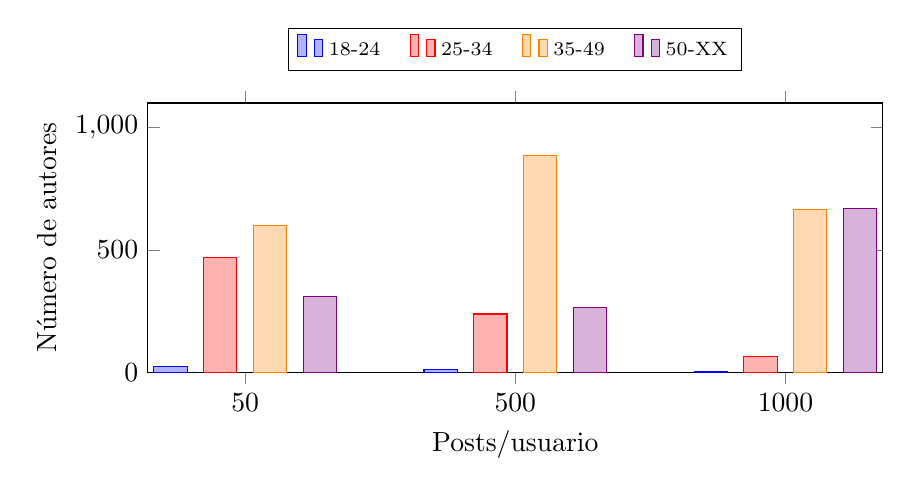
\begin{tikzpicture}
		\begin{axis}[
				width=0.9\textwidth,
				height=5cm,
				xmajorgrids=false,
				ylabel=Número de autores,
				xlabel=Posts/usuario,
				ybar=6pt,
				bar width=12pt,
				enlarge x limits=0.18,
				symbolic x coords={50, 500, 1000},
				xtick=data,
				ymin=0,
				ymax=1100,
				legend style={at={(0.5,1.28)},font=\scriptsize, anchor=north,legend columns=-1, /tikz/every even column/.append style={column sep=0.3cm}},
			]
			\addplot[color=blue, fill=blue!30] table[x=Posts/usuario,y={18-24}] {
			Posts/usuario   {18-24}
			50              24
			500             11
			1000            4
			};
			\addplot[color=red, fill=red!30] table[x=Posts/usuario,y={25-34}] {
			Posts/usuario   {25-34}
			50              470
			500             238
			1000            63
			};
			\addplot[color=orange, fill=orange!30] table[x=Posts/usuario,y={35-49}] {
			Posts/usuario   {35-49}
			50              600
			500             887
			1000            665
			};
			\addplot[color=violet, fill=violet!30] table[x=Posts/usuario,y={50-XX}] {
			Posts/usuario   {50-XX}
			50              308
			500             266
			1000            670
			};
			\legend{{18-24}, {25-34}, {35-49}, {50-XX}}
		\end{axis}
	\end{tikzpicture}
	\caption{Distribución de edad obtenida por el algoritmo de Martinc at al. \cite{martinc2019hot}}
	\label{fig:comparativa_edad_martinc}
\end{figure}

\bigskip
\begin{table}[H]
	\centering
	\resizebox{0.8\textwidth}{!}{
		\rowcolors{2}{white}{udcgray!25}
		\begin{tabular}{|c|c|c|c|c|c|}
			\hhline{~|-----|}
			\multicolumn{1}{c|}{\cellcolor{white}} & \multicolumn{5}{c|}{\cellcolor{udcpink!25}\textbf{Martinc}}                                                                     \\ \hline
			\textbf{Posts/usuario}                 & \textbf{XX-17}                                              & \textbf{18-24} & \textbf{25-34} & \textbf{35-49} & \textbf{50-XX} \\ \hline
			50                                     & 0                                                           & 24             & 470            & 600            & 308            \\ \hline
			500                                    & 0                                                           & 11             & 238            & 887            & 266            \\ \hline
			1,000                                  & 0                                                           & 4              & 63             & 665            & 670            \\ \hline
		\end{tabular}
	}
	\caption{Distribución de edad obtenida por el algoritmo de Martinc et al. \cite{martinc2019hot}}
	\label{tab:comparativa_edad_martinc}
\end{table}

\bigskip
Pasando al algoritmo de Grivas et al. \cite{grivas2015author}, y de la misma forma que sucedía con la distribución de género, los resultados obtenidos
parecen estar la mayor parte concentrados en dos clases, las cuales coinciden con las más representadas en la colección de entrenamiento para el algoritmo (ver Figura \ref{fig:dataset_2015}).
Esto denota, lógicamente, un claro sobreajuste del modelo a dicha colección. 
{\color{red}
A pesar de ello, todas estas inferencias desde los datos a nivel sociológico representan en sí mismo contribuciones de este TFG,
ya que abren nuevas hipótesis de trabajo acerca del fenómeno \#BLM.
}
\bigskip
\begin{figure}[H]
	\centering
	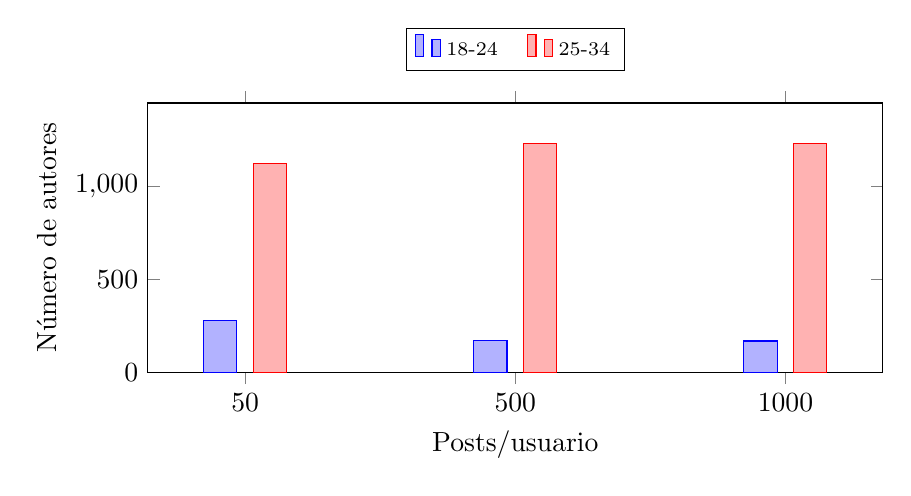
\begin{tikzpicture}
		\begin{axis}[
				width=0.9\textwidth,
				height=5cm,
				xmajorgrids=false,
				ylabel=Número de autores,
				xlabel=Posts/usuario,
				ybar=6pt,
				bar width=12pt,
				enlarge x limits=0.18,
				symbolic x coords={50, 500, 1000},
				xtick=data,
				ymin=0,
				ymax=1450,
				legend style={at={(0.5,1.28)},font=\scriptsize, anchor=north,legend columns=-1, /tikz/every even column/.append style={column sep=0.3cm}},
			]
			\addplot[color=blue, fill=blue!30] table[x=Posts/usuario,y={18-24}] {
			Posts/usuario   {18-24}
			50              278
			500             170
			1000            168
			};
			\addplot[color=red, fill=red!30] table[x=Posts/usuario,y={25-34}] {
			Posts/usuario   {25-34}
			50              1124
			500             1232
			1000            1234
			};
			\legend{{18-24}, {25-34}}
		\end{axis}
	\end{tikzpicture}
	\caption{Distribución de edad obtenia por el algoritmo de Grivas at al. \cite{grivas2015author}}
	\label{fig:comparativa_edad_grivas}
\end{figure}

\begin{table}[H]
	\centering
	\resizebox{0.8\textwidth}{!}{
		\rowcolors{2}{white}{udcgray!25}
		\begin{tabular}{|c|c|c|c|c|c|}
			\hhline{~|-----|}
			\multicolumn{1}{c|}{\cellcolor{white}} & \multicolumn{5}{c|}{\cellcolor{udcpink!25}\textbf{Grivas}}                                                                     \\ \hline
			\textbf{Posts/usuario}                 & \textbf{XX-17}                                             & \textbf{18-24} & \textbf{25-34} & \textbf{35-49} & \textbf{50-XX} \\ \hline
			50                                     & 0                                                          & 278            & 1.124          & 0              & 0              \\ \hline
			500                                    & 0                                                          & 170            & 1.232          & 0              & 0              \\ \hline
			1.000                                  & 0                                                          & 168            & 1.234          & 0              & 0              \\ \hline
		\end{tabular}
	}
	\caption{Distribución de edad obtenida por el algoritmo de Grivas et al. \cite{grivas2015author}}
	\label{tab:comparativa_edad_grivas}
\end{table}

\subsection{Otras características}

En lo que respecta al perfilado de los rasgos personales que ofrece el algoritmo de Grivas et al. \cite{grivas2015author},
lo primero que observamos es que existe muy poca variación con respecto al número de posts por usuario, como se puede ver en la Tabla \ref{tab:comparativa_rasgos_personales}.
A grandes rasgos, recordemos que los valores de cada rasgo personal oscilan entre -0,5 y 0,5, vemos como la característica que más destaca es claramente la de \textit{Open} (abierto a nuevas experiencias), seguida de \textit{Stable} (estable) y \textit{Agreeable} (amable).
Las implicaciones que tiene estos resultados con la realidad no son claras, pero podemos deducir que, en general, los usuarios que se lanzan a ser partícipes de los debates
en Reddit sobre el \#BLM son personas categorizadas en unos rasgos de personalidad abiertos y estables.

\bigskip
\begin{table}[H]
	\centering
	\resizebox{0.8\textwidth}{!}{
		\rowcolors{2}{white}{udcgray!25}
		\setlength{\tabcolsep}{8pt}
		\begin{tabular}{|c|c|c|c|c|c|}
			\hhline{~|-----|}
			\multicolumn{1}{c|}{\cellcolor{white}} & \multicolumn{5}{c|}{\cellcolor{udcpink!25}\textbf{Martinc}}                                                                                                                     \\ \hline
			\textbf{Posts/usuario}                 & \textbf{\textit{Extroverted}}                               & \textbf{\textit{Stable}} & \textbf{\textit{Agreeable}} & \textbf{\textit{Conscientious}} & \textbf{\textit{Open}} \\ \hline
			50                                     & 0,1630                                                      & 0,1956                   & 0,1877                      & 0,1787                          & 0,3271                 \\ \hline
			500                                    & 0,1536                                                      & 0,1974                   & 0,1968                      & 0,1771                          & 0,3349                 \\ \hline
			1,000                                  & 0,1529                                                      & 0,1972                   & 0,1969                      & 0,1769                          & 0,3358                 \\ \hline
		\end{tabular}
	}
	\caption{Distribución media de los rasgos personales obtenidos por el algoritmo de Grivas et al. \cite{grivas2015author}}
	\label{tab:comparativa_rasgos_personales}
\end{table}

Finalmente, en lo que respecta a las características únicas perfiladas por el algoritmo de Martinc et al. \cite{martinc2019hot}, es decir, la ocupación y el nivel de fama,
creemos que no aportan información relevante para este análisis, dado que son características pensadas
específicamente para el perfilado de celebridades. A pesar de ello, se pueden ver las distribuciones obtenidas en las
Tablas \ref{tab:comparativa_ocupacion_martinc} y \ref{tab:comparativa_fama_martinc}.

\bigskip
\begin{table}[H]
	\centering
	\resizebox{\textwidth}{!}{
		\rowcolors{2}{white}{udcgray!25}
		\setlength{\tabcolsep}{7pt}
		\begin{tabular}{|c|c|c|c|c|c|c|c|c|}
			\hhline{~|--------|}
			\multicolumn{1}{c|}{\cellcolor{white}} & \multicolumn{8}{c|}{\cellcolor{udcpink!25}\textbf{Martinc}}                                                                                                                                                                                                         \\ \hline
			\textbf{Posts/usuario}                 & \textbf{\textit{Professional}}                              & \textbf{\textit{Performer}} & \textbf{\textit{Science}} & \textbf{\textit{Politics}} & \textbf{\textit{Manager}} & \textbf{\textit{Creator}} & \textbf{\textit{Sports}} & \textbf{\textit{Religious}} \\ \hline
			50                                     & 4                                                           & 545                         & 37                        & 19                         & 4                         & 359                       & 434                      & 0                           \\ \hline
			500                                    & 0                                                           & 680                         & 34                        & 2                          & 1                         & 396                       & 289                      & 0                           \\ \hline
			1,000                                  & 2                                                           & 691                         & 73                        & 3                          & 1                         & 321                       & 311                      & 0                           \\ \hline
		\end{tabular}
	}
	\caption{Distribución de ocupación obtenida por el algoritmo de Martinc et al. \cite{martinc2019hot}}
	\label{tab:comparativa_ocupacion_martinc}
\end{table}

\bigskip
\begin{table}[H]
	\centering
	\resizebox{0.6\textwidth}{!}{
		\rowcolors{2}{white}{udcgray!25}
		\begin{tabular}{|c|c|c|c|}
			\hhline{~|---|}
			\multicolumn{1}{c|}{\cellcolor{white}} & \multicolumn{3}{c|}{\cellcolor{udcpink!25}\textbf{Martinc}}                                                        \\ \hline
			\textbf{Posts/usuario}                 & \textbf{\textit{Rising}}                                    & \textbf{\textit{Star}} & \textbf{\textit{Superstar}} \\ \hline
			50                                     & 2                                                           & 1.202                  & 198                         \\ \hline
			500                                    & 1                                                           & 1.226                  & 175                         \\ \hline
			1.000                                  & 1                                                           & 1.261                  & 140                         \\ \hline
		\end{tabular}
	}
	\caption{Distribución de fama obtenida por algoritmo de Martinc et al. \cite{martinc2019hot}}
	\label{tab:comparativa_fama_martinc}
\end{table}
